\documentclass[]{article}
\usepackage{lmodern}
\usepackage{amssymb,amsmath}
\usepackage{ifxetex,ifluatex}
\usepackage{fixltx2e} % provides \textsubscript
\ifnum 0\ifxetex 1\fi\ifluatex 1\fi=0 % if pdftex
  \usepackage[T1]{fontenc}
  \usepackage[utf8]{inputenc}
\else % if luatex or xelatex
  \ifxetex
    \usepackage{mathspec}
  \else
    \usepackage{fontspec}
  \fi
  \defaultfontfeatures{Ligatures=TeX,Scale=MatchLowercase}
\fi
% use upquote if available, for straight quotes in verbatim environments
\IfFileExists{upquote.sty}{\usepackage{upquote}}{}
% use microtype if available
\IfFileExists{microtype.sty}{%
\usepackage{microtype}
\UseMicrotypeSet[protrusion]{basicmath} % disable protrusion for tt fonts
}{}
\usepackage[margin=1in]{geometry}
\usepackage{hyperref}
\hypersetup{unicode=true,
            pdftitle={Target-based site prioritization under climate change using quadratic network flow},
            pdfauthor={Derek Corcoran},
            pdfborder={0 0 0},
            breaklinks=true}
\urlstyle{same}  % don't use monospace font for urls
\usepackage{longtable,booktabs}
\usepackage{graphicx,grffile}
\makeatletter
\def\maxwidth{\ifdim\Gin@nat@width>\linewidth\linewidth\else\Gin@nat@width\fi}
\def\maxheight{\ifdim\Gin@nat@height>\textheight\textheight\else\Gin@nat@height\fi}
\makeatother
% Scale images if necessary, so that they will not overflow the page
% margins by default, and it is still possible to overwrite the defaults
% using explicit options in \includegraphics[width, height, ...]{}
\setkeys{Gin}{width=\maxwidth,height=\maxheight,keepaspectratio}
\IfFileExists{parskip.sty}{%
\usepackage{parskip}
}{% else
\setlength{\parindent}{0pt}
\setlength{\parskip}{6pt plus 2pt minus 1pt}
}
\setlength{\emergencystretch}{3em}  % prevent overfull lines
\providecommand{\tightlist}{%
  \setlength{\itemsep}{0pt}\setlength{\parskip}{0pt}}
\setcounter{secnumdepth}{5}
% Redefines (sub)paragraphs to behave more like sections
\ifx\paragraph\undefined\else
\let\oldparagraph\paragraph
\renewcommand{\paragraph}[1]{\oldparagraph{#1}\mbox{}}
\fi
\ifx\subparagraph\undefined\else
\let\oldsubparagraph\subparagraph
\renewcommand{\subparagraph}[1]{\oldsubparagraph{#1}\mbox{}}
\fi

%%% Use protect on footnotes to avoid problems with footnotes in titles
\let\rmarkdownfootnote\footnote%
\def\footnote{\protect\rmarkdownfootnote}

%%% Change title format to be more compact
\usepackage{titling}

% Create subtitle command for use in maketitle
\providecommand{\subtitle}[1]{
  \posttitle{
    \begin{center}\large#1\end{center}
    }
}

\setlength{\droptitle}{-2em}

  \title{Target-based site prioritization under climate change using quadratic network flow}
    \pretitle{\vspace{\droptitle}\centering\huge}
  \posttitle{\par}
    \author{Derek Corcoran}
    \preauthor{\centering\large\emph}
  \postauthor{\par}
    \date{}
    \predate{}\postdate{}
  
\usepackage{booktabs}
\usepackage{longtable}
\usepackage{array}
\usepackage{multirow}
\usepackage{wrapfig}
\usepackage{float}
\usepackage{colortbl}
\usepackage{pdflscape}
\usepackage{tabu}
\usepackage{threeparttable}
\usepackage{threeparttablex}
\usepackage[normalem]{ulem}
\usepackage{makecell}
\usepackage{xcolor}

\begin{document}
\maketitle

\hypertarget{introduction}{%
\section{Introduction}\label{introduction}}

Currently, 14.9\% of terrestrial area is a part of the global protected area network (UNEP-WCMC, 2018). However, most of this areas have not been created using priorization tools developed to maximize species or ecosystems conservation based on current biodiversity patterns (Rodrigues et al., 2004; Jenkins, Van Houtan, Pimm, \& Sexton, 2015). The situation is even worst when we take into account that the range of species will change over time (Araújo, Cabeza, Thuiller, Hannah, \& Williams, 2004; Lenoir, Gégout, Marquet, De Ruffray, \& Brisse, 2008; Chen, Hill, Ohlemüller, Roy, \& Thomas, 2011; Regos et al., 2016), were several species that are now being protected by these areas might not be protected in the future because of the climate crisis (Araújo et al., 2004; Alagador, Cerdeira, \& Araújo, 2014).

Despite the concern about protected area planning, a review Jones, Watson, Possingham, \& Klein (2016) shows that more than 90\% of the prioritization planing studies that try to incorporate climate change, only take two time steps into account, current climate and the last step of climate. Currently, two of the most used tools for conservation planning are Prioritize and Zonation (Di Minin et al., 2014; Hanson et al., 2019). Zonation can be used for conservation prioritization under climate change as conservation features may be explicitly linked through interaction. This allows for simultaneous prioritization of a species current range, its modelled future range, and the connectivity between the two limited by a species' capacity to disperse.

\begin{table}[H]
\centering
\begin{tabular}{lllll}
\toprule
 & Network flow & Zonation & Migclim & Prioritizr\\
\midrule
Considers more than 2 time-slices & Yes & No & Yes & No\\
Can add species to the solutions afterwards & Yes & No & Yes & No\\
Keep track of species dispersal routes & Yes & Yes & Yes & No\\
Solves for conservation targets & Yes & Yes & No & Yes\\
Considers cost as part of the solution & Yes & Yes & No & Yes\\
\bottomrule
\end{tabular}
\end{table}

However, in order for the species to move from areas were they are currently protected to the future protected areas, their route has to be protected as well, that is the biological corridors that they will use (Rosenberg, Noon, \& Meslow, 1997; Nuñez et al., 2013). Thus, the planification and creation of those biological corridors correspond to adaptive measures to environmental changes that would mitigate the impacts of the climate crisis (Hannah et al., 2007). In that context, biological corridors should consider effects of climate crisis, changes in land use and habitat fragmentation, in order to evaluate the factibility of the species reaching future available habitat.

There have been several approaches trying to model biological corridors. Local approaches have focus just in one or a few species (Cushman et al., 2013; Alagador et al., 2014; Gregory et al., 2014) or group of species (Williams et al., 2005; Beier, Majka, \& Bayless, 2007; Phillips, Williams, Midgley, \& Archer, 2008), not being able to be use for planning for lack of species or be in confined spaces, respectively. A continental approach was made by Lawler, Ruesch, Olden, \& McRae (2013), who modelled biological corridors in the Americas. Even when that model was made for close to 3,000 species did not consider species dispersal speed or use the information to build priority areas. Among these articles, the work of Phillips et al. (2008), incorporates the use of the Network Flow optimization method (Ahuja, Magnanti, \& Orlin, 1993) in order to solve the problem expressed by Williams et al. (2005), generating a solution 33\% more efficient than previous optimization methods. This makes this methodology one of the most promising ways of solving conservation planning problems through the use of biological corridors.

In its traditional use, Network flow gives the best possible solution given constrains (Phillips et al., 2008). If we looked at the solution for a species in a raster, every cell would have a value of either one or zero, where one would be a cell necessary for the conservation of the species or a zero if it is not necessary. This best solution, however, only represents one of the possible solutions to conserve a species, and does not give us any alternatives. in this research we present Quadratic Cost Network Flow as alternative solution, where for every species we would still get a value of one if the cell is irreplaceable for the solution, zero if that cell is not needed, and an intermediate value for cells that are one of many alternative solutions for a given species, this is, for every cell we have an irreplaceability index. Spatial planning is a complex endeavour where agendas and/or needs evolve rapidly and several alternative suboptimal solutions might be needed in order to navigate this complex decisions.

In this article we present a new method of working with network flow on conservation planning using quadratic costs, while at the same time comparing its results and implications with traditional network flow and zonation, using the Northern Tropical Andes ecorregion as an example.

\hypertarget{methods}{%
\section{Methods}\label{methods}}

\hypertarget{area}{%
\subsection{Area}\label{area}}

The studied area was the Northern Tropical Andes, consisting of the countries of Colombia, Venezuela and Ecuador, with a buffer of 200 kilometres around land areas.

\begin{figure}

{\centering 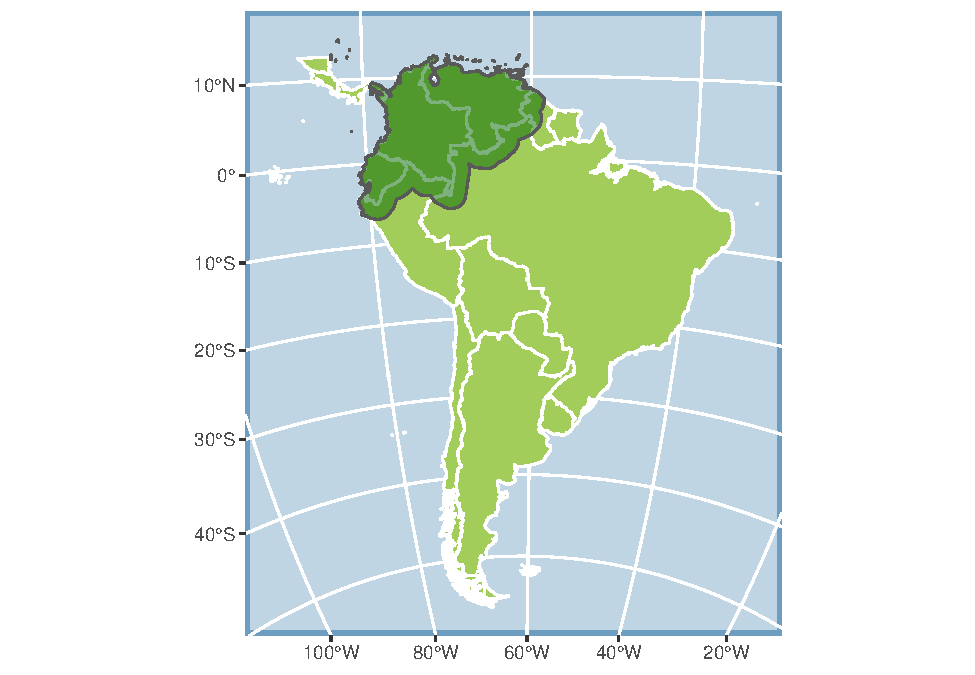
\includegraphics{NFPaper_files/figure-latex/MapArea-1} 

}

\caption{Map of Southamerica, the darkened area is the area where the priorization was performed}\label{fig:MapArea}
\end{figure}

The studied area is shown in figure \ref{fig:MapArea} and it encompasses 3,632,762 square kilometres

\hypertarget{species}{%
\subsection{Species}\label{species}}

671 species of plants and vertebrates were used for the model, only endemic species were used in this study. A list can be found in the supplementary materials

\hypertarget{global-circulation-models}{%
\subsection{Global circulation models}\label{global-circulation-models}}

Global Circulation Models (GCMs) are predictive models that use fluid models\ldots{} In order to select 4 GCMs, GCMComparer application was used \ref{fig:Diagrama}. Distribution models were generated for each GCM using the Dismo Package in R. Then, each model was projected as a binary response (presence-absence) for all decades form 2000 (present) to 2070 completing 8 time slices for each species.

For each species, a network of dispersion into each time-slice was generated using the QuadCostAmpl package, and finally we solved for Network Flow using the AMPL software using the Gurobi solver

\begin{figure}
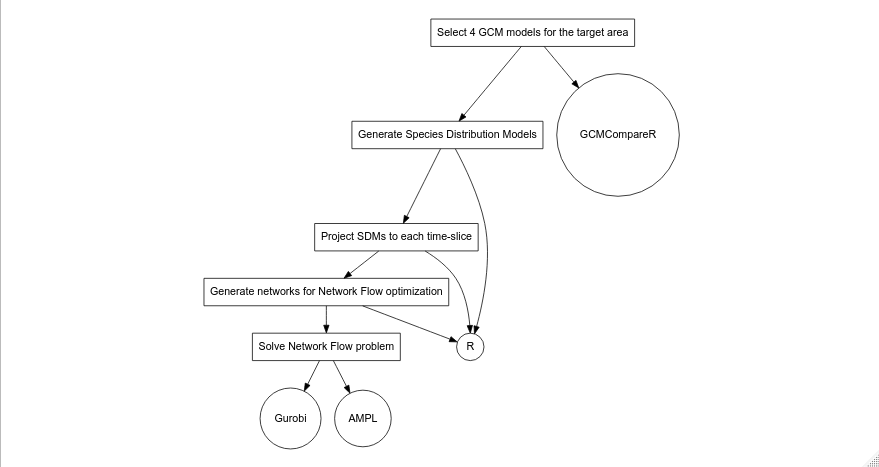
\includegraphics[width=4.39in]{Diag1} \caption{All the steps and programs used in the Optimization}\label{fig:Diagrama}
\end{figure}

Four GCM models were selected to project the species distribution using the GCMcompareR shiny app (Fajardo, Corcoran, Roehrdanz, Hannah, \& Marquet, 2018), we followed the story-lines approach (Zappa \& Shepherd, 2017) and selected a GCM warmer and wetter, warmer and dryer, colder and wetter, and colder and dryer than the ensemble. The selected models where cc, cn, la, mp al the process is shown in in figure \ref{fig:Diagrama}.

\hypertarget{niche-modelling}{%
\subsection{Niche modelling}\label{niche-modelling}}

\hypertarget{bien-data-standardization-workflow.}{%
\subsubsection{BIEN Data Standardization Workflow.}\label{bien-data-standardization-workflow.}}

The BIEN database is generated via a linked workflow that imports and integrates heterogeneous data structures (including (Baker, Rycroft, \& Smith, 2014), plus a variety of project-specific schemas and exchange formats), and then performs multiple corrections and validations. The BIEN workflow is described at \url{http://bien.nceas.ucsb.edu/bien/tools/} and in the following references (49-53). In addition to correcting erroneous original content and standardizing variant spellings to a single canonical form, corrections also remove or flag erroneous content when the correct meaning cannot be determined). Validations delete erroneous records and add annotations that can be used to filter low-quality data and data useful for some analyses but not others (e.g., observations of introduced or cultivated species).

The two major classes of corrections are taxonomic name resolution and geographic name resolution. Taxonomy is standardized using the Taxonomic Name Resolution Service (Boyle et al., 2013), which corrects spelling errors in scientific names, standardizes variant spelling and updates synonyms to accepted names. Additional code detects cross-code homonyms (e.g.~plant and animal species with identical names) and flags non-plant observations for removal. The names of political divisions (e.g.~country, state/ province, county/parish) are standardized using the Geographic Name Resolution Service (Boyle, 2019a) which corrects spelling errors and matches codes (e.g., ISO, FIPS), abbreviations, variant spellings and alternative names in multiple languages to standard political divisions in the GeoNames gazetteer (\url{https://www.geonames.org}).

The two major classes of validations are geographic validation and species status validation. Checks performed by geographic validations include (1) coordinate values outside coordinate system (e.g., longitudes larger than 180 degrees or smaller than -180), (2) likely erroneous coordinate values (latitude is exactly 0 or 90 or longitude is exactly 0 or 180, (3) coordinates in the ocean, (4) coordinate matches a centroid (centroid detection) and (5) coordinates outside lowest declared political division (political division validation). Centroid detection and political division validation used administrative boundaries from the Database of Global Administrative Areas (GADM; \url{http://www.gadm.org}), with political division names standardized by the GNRS (see above). Species status validations checked for (1) species falling outside their native ranges and (2) observations of human-cultivated plants. Observations species outside of their native range were identified using the Native Species Resolver (Boyle, 2019b), which uses published country and state checklists to determine if the observed species is native to the lowest declare political divisions. List of endemic taxa are also used to detect non-native occurrences outside the region of endemism. and endemism data. Observations were flagged as cultivated based on (1) keywords in the specimen locality data suggesting provenance from a farm or garden, or (2) geographic proximity (\(\leq\) 3 km) to a botanical garden or herbarium, or (3) original observation metadata indicating a cultivated origin.

For these analyses we excluded records if (1) they lacked a scientific name resolved to at least the species level; (2) they did not come from a land plant (Embryophyta); (3) they failed one or more geographic validations; (4) the species was flagged as potentially non-native to the region of observation; (5) the plant was flagged as potentially cultivated; 5) the observation did not originate from either plot or specimen data.

\hypertarget{vertebrates.}{%
\subsubsection{Vertebrates.}\label{vertebrates.}}

Point occurrences for global restricted range bird species (61). Point occurrences for tropical vertebrates (GBIF, VertNet). Occurrences with geovalid coordinates. Occurrences more recent than 1950. Human observations only (no fossil records or museum specimens). Political centroids and locations with zeros removed. Spatial outliers -- more than 500km from IUCN range polygon or \textgreater{}98th percentile of latitude + longitude. Expert range maps polygons for all available mammals, birds, reptiles were used as a means of model and occurrence record validation (61-62)

\hypertarget{species-distribution-models.}{%
\subsubsection{Species Distribution Models.}\label{species-distribution-models.}}

Species distribution models were produced with Maxent (Phillips, Anderson, \& Schapire, 2006; Merow, Smith, \& Silander Jr, 2013) using the Dismo Package (Hijmans, Phillips, Leathwick, \& Elith, 2017) for species with over 10 unique occurrence records (i.e.~unique 1km grid cells in the modelling domain). Maxent settings followed the recommendations of Merow et al. (2013) and Merow et al. (2014) to produce relatively less complex models (e.g.~limiting features to linear, quadratic, and product functions) to minimize overfitting. Modeling domains were limited to a spatial buffer of 500km within any geovalid occurrence record. Background sampling for pseudoabsence point was a random sample of 50,000 points. Five model replicates were used in fitting the model. Average of five replicates was used for final species model in baseline climate -- and those fitted parameters were used for all projections into future climates. 30\% of occurrence records were reserved to assess model performance.

Environmental Predictor Variables. The following bioclimatic variables from downscaled 20-year normals (66) based on pan-tropical correlation analysis and ability to describe the climate for a given location. When presented with the choice of two variables that were otherwise closely correlated, we selected the variable that were not combinations of temperature and precipitation or relied on monthly segmentation of the yearly climate (e.g.~precipitation in the warmest quarter).

\begin{itemize}
\tightlist
\item
  Mean annual temperature (BIO1)
\item
  Mean diurnal temperature range (BIO2)
\item
  Seasonality of temperature (BIO4)
\item
  Minimum temperature of the coldest month (BIO6)
\item
  Mean annual precipitation (BIO12)
\item
  Seasonality of precipitation (BIO15)
\end{itemize}

Accumulated Aridity Index. To account for the effect of dry season length and the water deficit experienced by vegetation during dry periods we derived and accumulated aridity index that identifies the maximum duration and accumulated water deficit for consecutive months where potential evapotranspiration exceeds mean monthly precipitation. The accumulated aridity index is the sum of the month aridity (precipitation -- PET) for the maximum run of consecutive months where (PET \textgreater{} precipitation).

Soils Variables. The following soils variables were also used in species distribution models. All variables were obtained from Soilgrids (De Sousa, Heuvelink, Batjes, \& Kempen, 2018). Variables with multiple strata available are the mean of the top 1m (strata 1-4).

\begin{itemize}
\tightlist
\item
  depth to bedrock
\item
  pH
\item
  clay proportion\\
\item
  silt proportion
\item
  bulk density
\end{itemize}

Prioritization under Climate Change. Zonation Conservation Planning Software is a widely used tool that allows for simultaneous prioritization of many thousands of conservation features (i.e.~species or ecosystem types) while also considering fundamental aspects of the landscape including habitat condition, connectivity, and cost (68-69). Zonation can be used for conservation prioritization under climate change as conservation features may be explicitly linked through interaction. This allows for simultaneous prioritization of a species current range, its modeled future range, and the connectivity between the two limited by a species' capacity to disperse. The protocol for running Zonation under uncertain climate change projections is thoroughly described in Kujala et al.~2013 (70).

Species current ranges were linked to projected future ranges through an interaction layer. This layer is transformed by a dispersal kernel with a parameter to limit the interaction to the species total capacity to disperse over the period of analysis. Total dispersal capacity was assumed to be 100km for vertebrates (roughly 1 km/yr) and 1km for vascular plants (roughly 100m/yr). The algorithm favors areas of the species range in baseline climate that are retained in the projected future climate (i.e.~the areas are suitable for species in both baseline and future climate). Prioritization were conducted using the mean projected future species ranges across 10 GCM under the same RCP (RCP2.6 or RCP8.5) that were discounted by the standard deviation the projected ranges. Prioritizations were also run for each GCM individually for both RCP2.6 and RCP8.5

Conservation Features. All available species models (vascular plants and vertebrates) were used in continental scale prioritizations. Prioritization used the continuous value output of species distribution models for current climates and projected future climates. See species distribution modeling section above for more information. Models were fit at 30 arc-second resolution and were projected into 5km resolution environmental layers. All available species models (vascular plants and vertebrates) were used in continental scale prioritizations. Species with too few occurrence records to produce a model were included as point locations (Zonation term = ``Species of Special Interest''). Equal weighting was used for all conservation features.

\hypertarget{prioritization-methods.}{%
\subsubsection{Prioritization Methods.}\label{prioritization-methods.}}

Zonation ranks all cells in a landscape according to their value and removes cells of lowest value at each processing step. Values are then recalculated for all remaining cells at each step. Core area zonation removal algorithm was used this assigns value to a cell from the highest value species present in that cell at each step of removal. Species with smaller ranges have few cells that are critical for their conservation these cells therefore tend to have high values. By contrast, wide ranging species have more opportunities to be conserved -- so are typically lower value until only the core range remains. Warp factor (number of cells removed at each step) for all analysis was set to 1 to maximize the accuracy of the rank order assigned. All prioritizations used edge removal and boundary length penalty of 1.

Land Cover and Land Use. Areas of existing built up land or intensive agriculture were removed from the analysis and therefore those cells are not part of the prioritization solution. Built up and agricultural areas were defined as \textgreater{}50\% of pixel coverage for `urban' and `agriculture' classes from the 1km global consensus land cover dataset produced by Tuanmu et al.~2014 (71). Existing protected areas (40) are solved first so that the priorities take existing protection into account.

\hypertarget{cost-layer}{%
\subsection{Cost layer}\label{cost-layer}}

We used a 2.5 minutes downscaled version of Naidoo \& Iwamura (2007) layer of costs in order to estimate the cost per hectare for each area, and then we modified that layer using the World Database on Protected Areas (WDPA) (UNEP-WCMC, 2018), and land-cover (Tuanmu \& Jetz, 2014). If a cell of the cost layer was inside a proteced area, this was multiplied by zero, and if it was outside of a protected area it was multiplied by one.

\hypertarget{model-description}{%
\subsection{Model Description}\label{model-description}}

This model was developed based on the notion of non-overlapping dispersal chains (Williams et al., 2005), and instead of having a binary solution (to protect or not protect an area), the result will be an index of importance going from zero to one. Here, zero means that there are no chains passing by that spacial point that go from the source to the final destination, and one is a point where chains have to pass through to reach the desired flow.
In order to do this, we follow Network-flow methods (Ahuja et al., 1993) to model the survival and dispersion of species along the space and time, using species distribution models and quadratic flow costs to split the flow evenly across alternative paths. Therefore, the resulting flow across an arc is high only if there are few alternatives to use that edge to achieve the target flow.
Even when model takes into account protected areas (cost zero) and human habitat such as cities (cost infinite) in the decision making, both were not included in this exercise to simplify the examples. This is a generalist model which only needs the distribution model of the species projected to each time slice and the maximum dispersal distance for each species.

\hypertarget{model-formulation}{%
\subsubsection{Model Formulation}\label{model-formulation}}

The objective is to minimize the cost

\(\underset{Quadcost}{\text{minimize}}\)

\[\small Quadcost =  \sum_{i=1}^n{(Cost\times Flow_t)^2}\]

\(\text{subject to}\)

\[\small \text{Initial Flow} = \sum_{i=1}^n{Flow_{t_1}} = \text{Target paths}\]

\[\small \text{Final Flow} = \sum_{i=1}^n{Flow_{t_{final}}} = \text{Target paths}\]

\[\small \text{Flow capacity} = \sum_{i=1}^n{Flow_{(i,t)}} \leq capacity_{(i,t)}\]

\hypertarget{network-generation}{%
\subsection{Network generation}\label{network-generation}}

In order to generate the networks de QuadCostAmpl package was used (Corcoran \& Fajardo, 2019)

\hypertarget{linear-network-flow}{%
\subsection{Linear Network Flow}\label{linear-network-flow}}

Model

\hypertarget{quadratic-network-flow}{%
\subsection{Quadratic Network Flow}\label{quadratic-network-flow}}

\hypertarget{zonation}{%
\subsection{Zonation}\label{zonation}}

\hypertarget{results}{%
\section*{Results}\label{results}}
\addcontentsline{toc}{section}{Results}

\begin{figure}
\centering
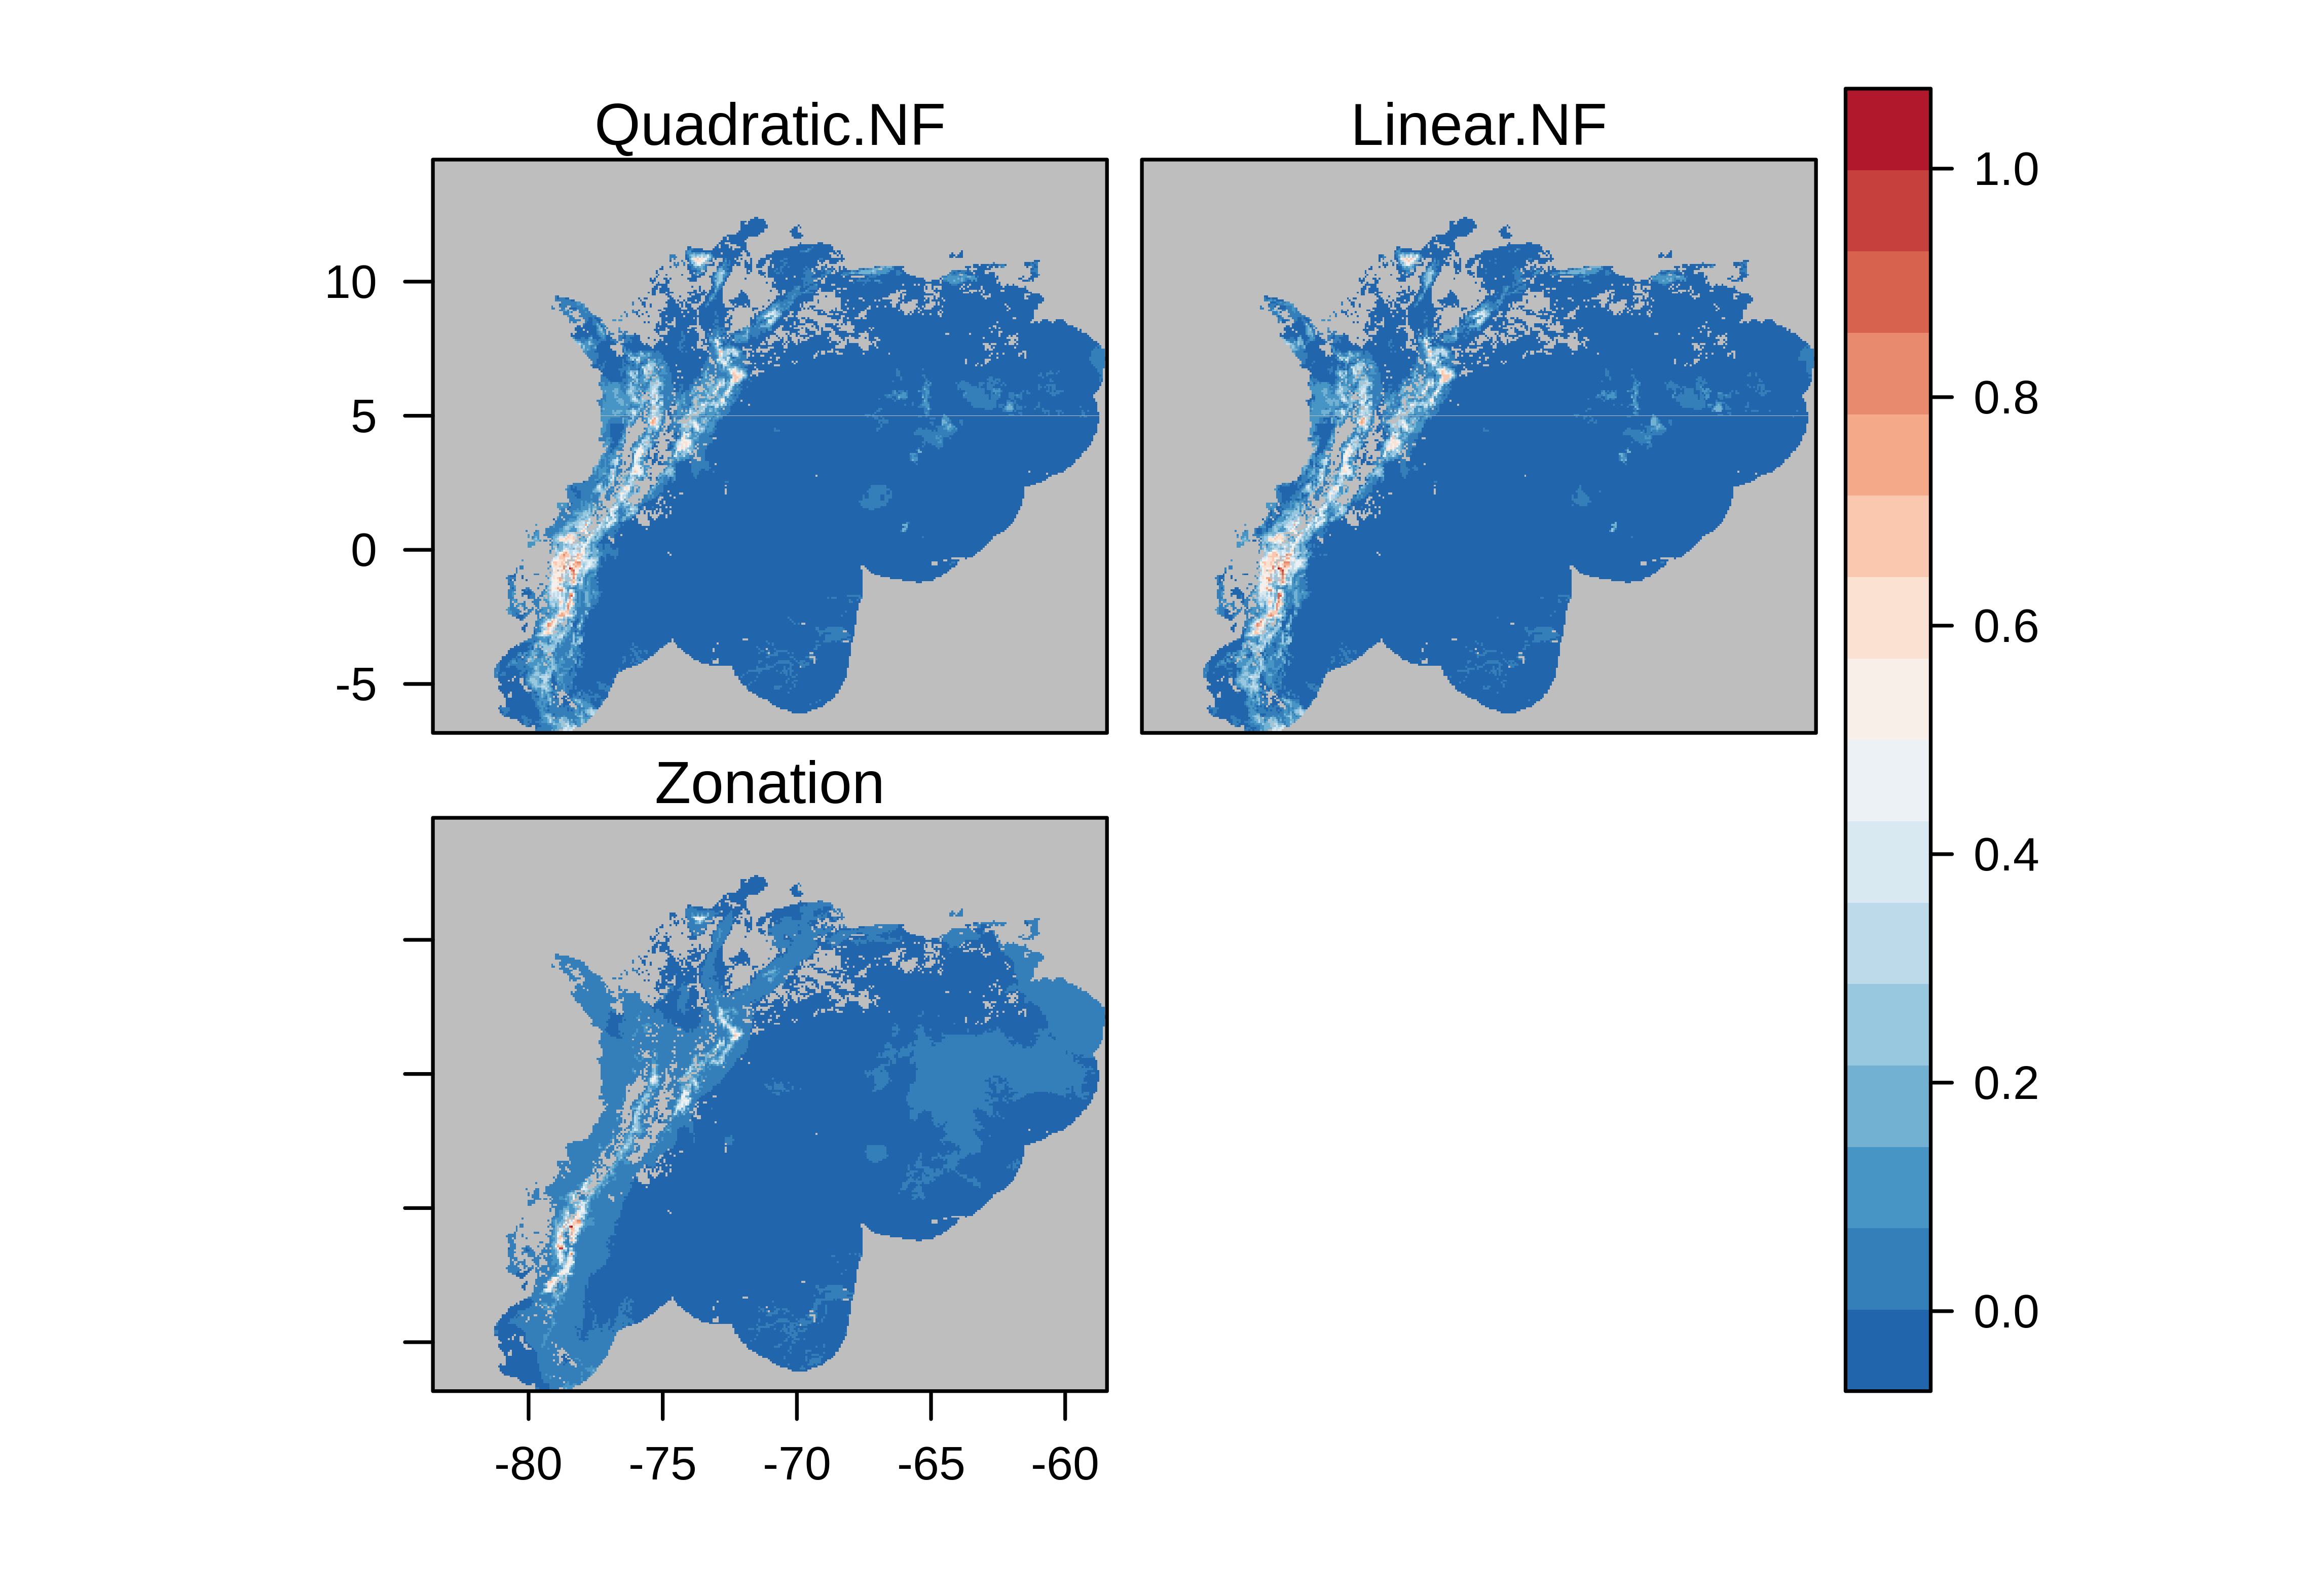
\includegraphics{NFPaper_files/figure-latex/AllSols-1.png}
\caption{\label{fig:AllSols}Coninuous results of the three algorithms, the highest the value the higher the priority, all values go from 0 to 1.}
\end{figure}

\begin{itemize}
\tightlist
\item
  \textbf{For methods:} Since one of the main objectives of priorization methods is to rank the cells within an area, we used Spearman's rho correlation, that estimates the rank-based measure of association. We also calculated a local Spearman correlation on a matrix of five by five cells, in order to figure out if there are some important
\end{itemize}

There are two ways of trying to look at the results, as a continuous layer, as in figure \ref{fig:AllSols}, or as a binary solution as in fig \ref{fig:Binary}, where the cells in red are the top 10\% ranked cells to be protected. At first glance, the three algorithms have very similar results. In all three methods the Andes mountains appear to have the highest priorities in particular the Northwest Andean montane forests, Eastern Cordillera Real montane forests, Venezuelan Andes montane forests, Cordillera Oriental montane forests, and the Cauca and Magdalena Valley montane forests, outside of the Andes mountains the ecorregions that have the highest priorities are Guianan Highlands moist forests, Pantepui forests \& shrub-lands and Cordillera La Costa montane forests. Furthermore, when we look at the top 10\% cells selected by the algorithms (Figures \ref{fig:Binary} and \ref{fig:NumberOfTimes}), we see that of all the cells that were selected at least by one algorithm 62.91\% of the cells were selected by all three algorithm, which show the level of concordance between cells, 18.85\% were selected by two of the algorithms and only 18.24\% of the cells selected were chosen by only one of the methods.

However, when we look at the Spearman correlation (table \ref{tab:Corr}), of all three methods we start seeing some important differences, where Quadratic and Linear Network flow have a spearman correlation of 0.92, but both methods have a smaller correlation with zonation, with Quadratic Network Flow having a higher correlation of 0.669, vs linear network flow having a correlation of 0.624 with Zonation. When we look at the local correlation plots (figure \ref{fig:LocalCorr}), we see that for the most part, the local correlations are all mostly positive, specially between both Network Flow algorithms. There are some blue areas in the figure, when comparing those priorities with zonation. Representing some big discrepancies in local prioritization, that is mostly localized

when we look at the box-plot of local correlation values (figure \ref{fig:Boxplot}), we see that the lower whiskers in the comparison of both Network Flow methods with Zonation, are bellow zero

\begin{itemize}
\tightlist
\item
  \textbf{For discussion:} One of the main problems at comparing Network Flow vs Zonation, is that Zonation will give a rank to each and every cell in the study area, which is not true for Network Flow. It comes as no surprise that Quadratic Network flow has a higher correlation with Zonation than Linear Network flow, the intended result of quadratic network flow being more similar to zonation than linear network flow.
\end{itemize}

\hypertarget{efficiency-comparison-number-of-cells}{%
\subsubsection{Efficiency comparison (Number of cells)}\label{efficiency-comparison-number-of-cells}}

\begin{figure}
\centering
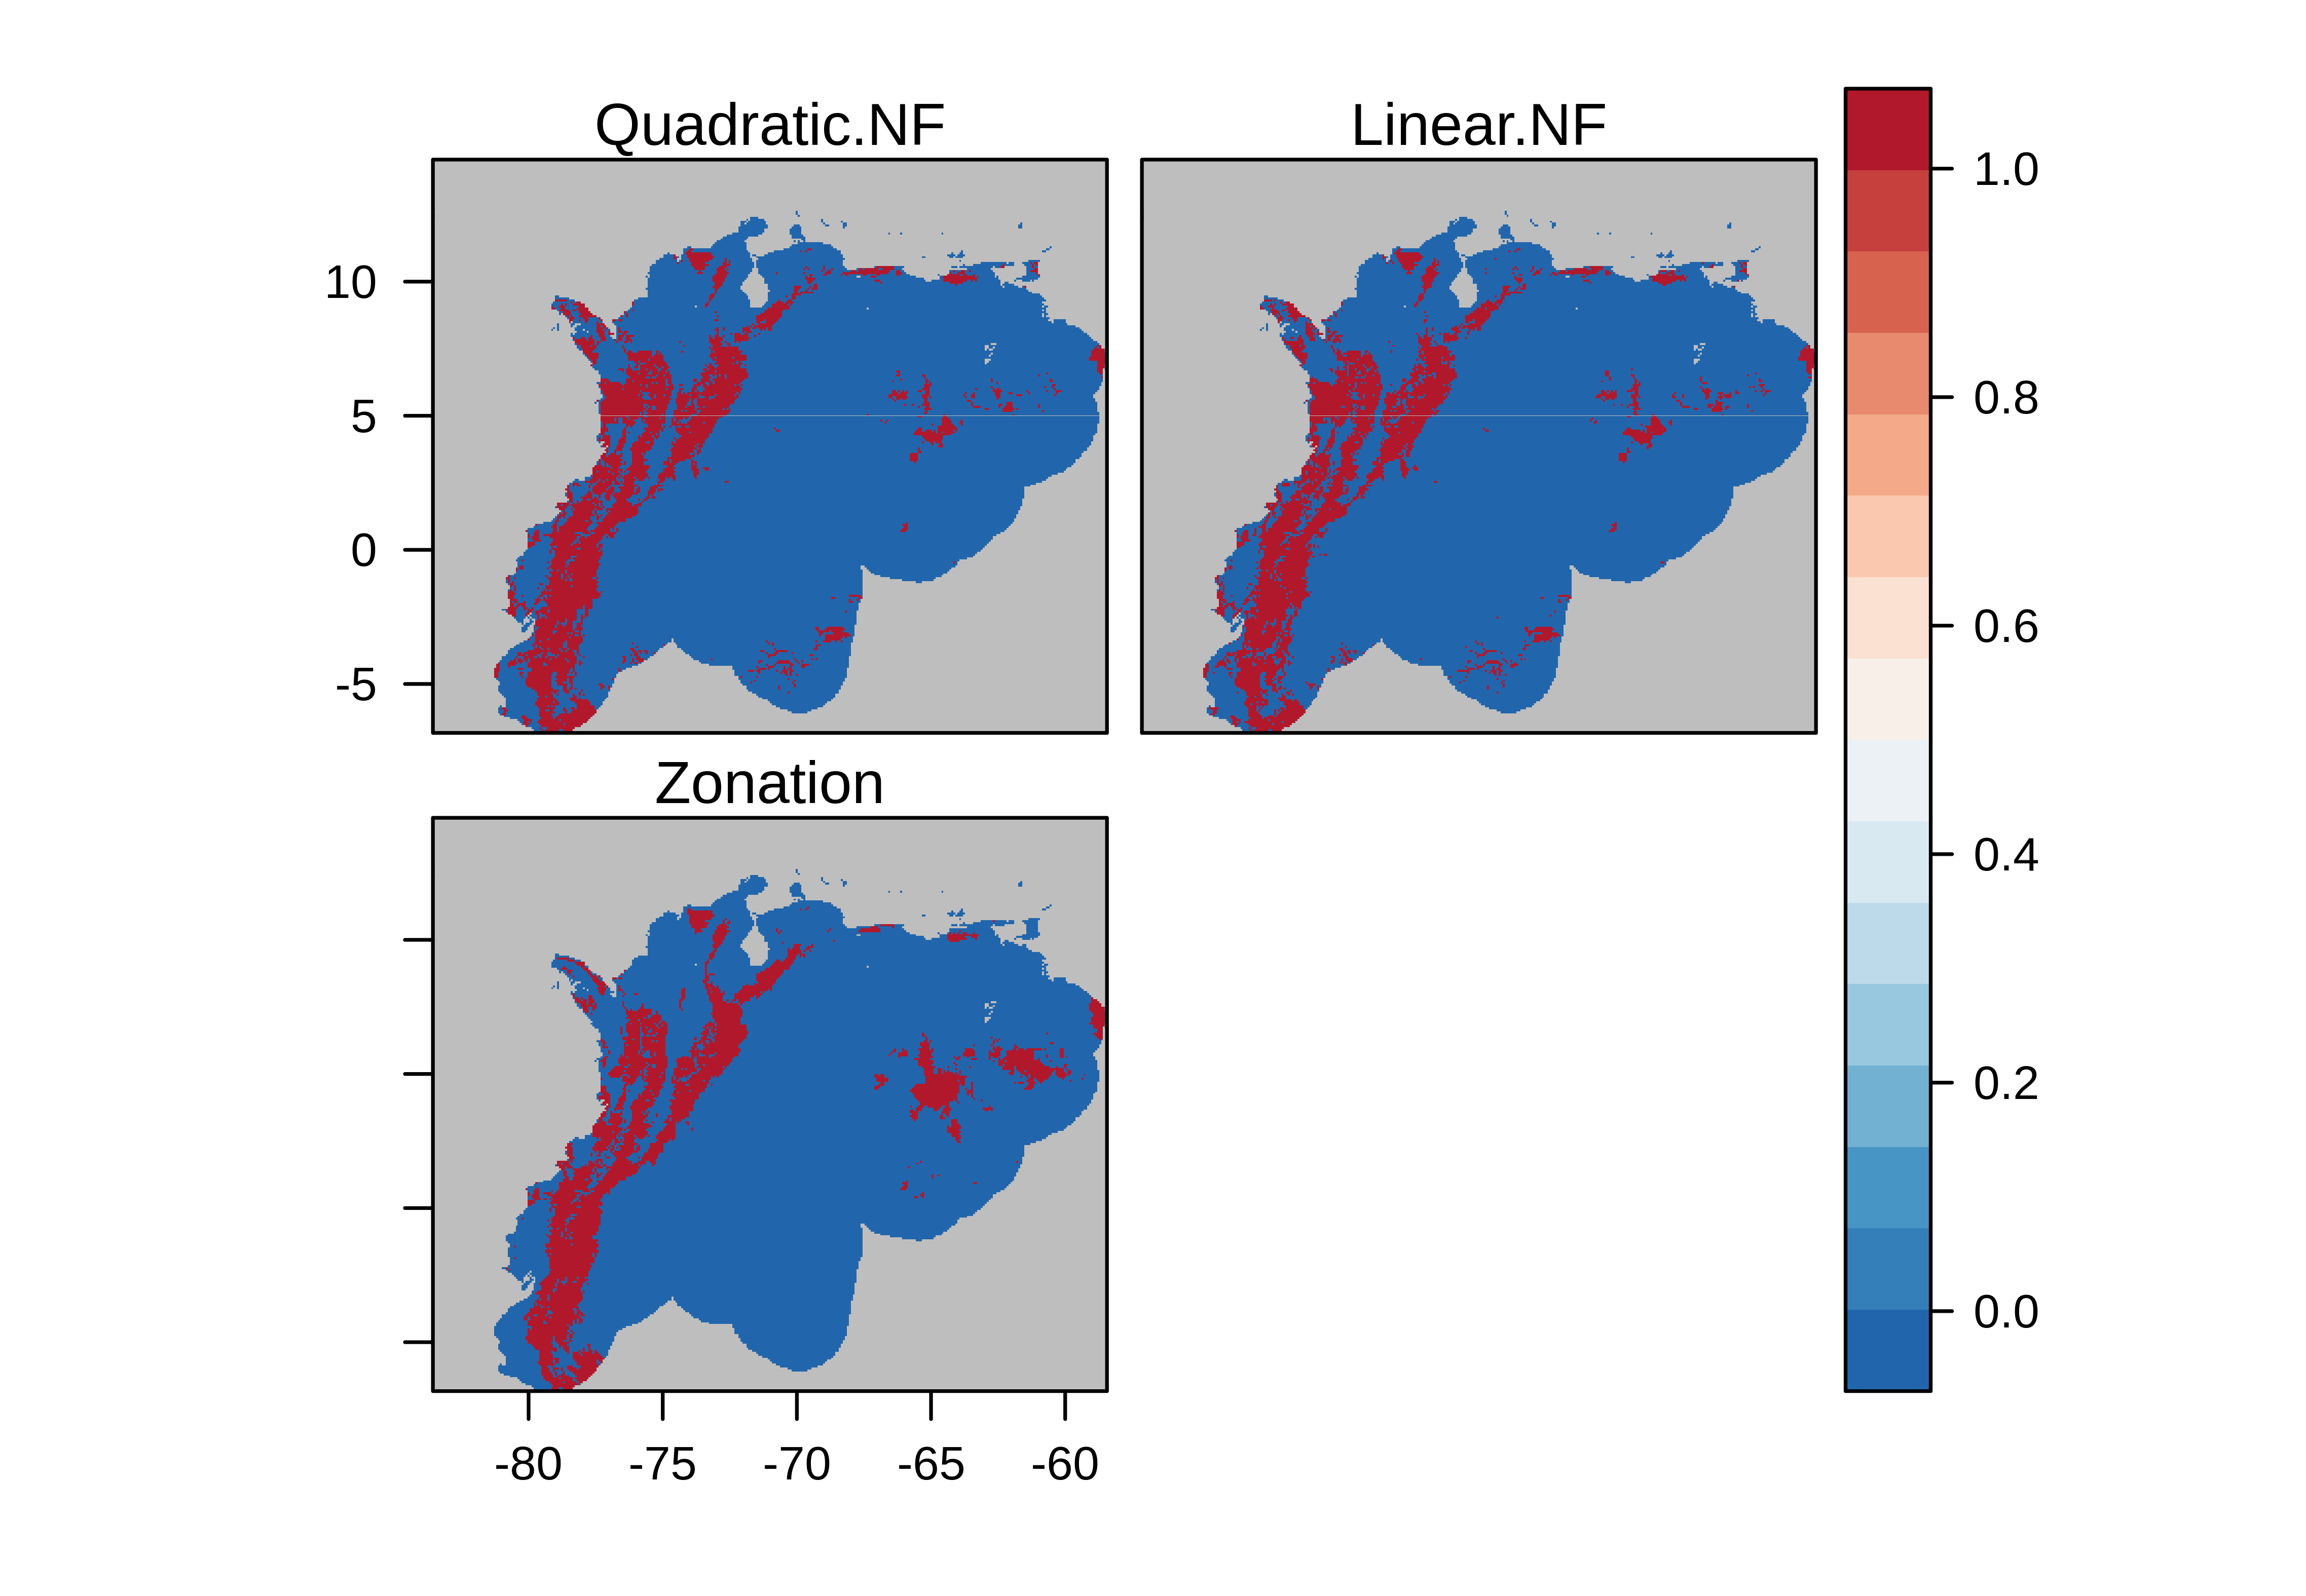
\includegraphics{NFPaper_files/figure-latex/Binary-1.png}
\caption{\label{fig:Binary}Binary solution for the cells with the top 10\% value of ranked priority}
\end{figure}

In this example when we calculate the top 10\% of protected cells for Quadratic Network Flow we get 22,671 cells, 22,586 cells for linear Network Flow, and 22,671 cells for Zonation.

\begin{figure}
\centering
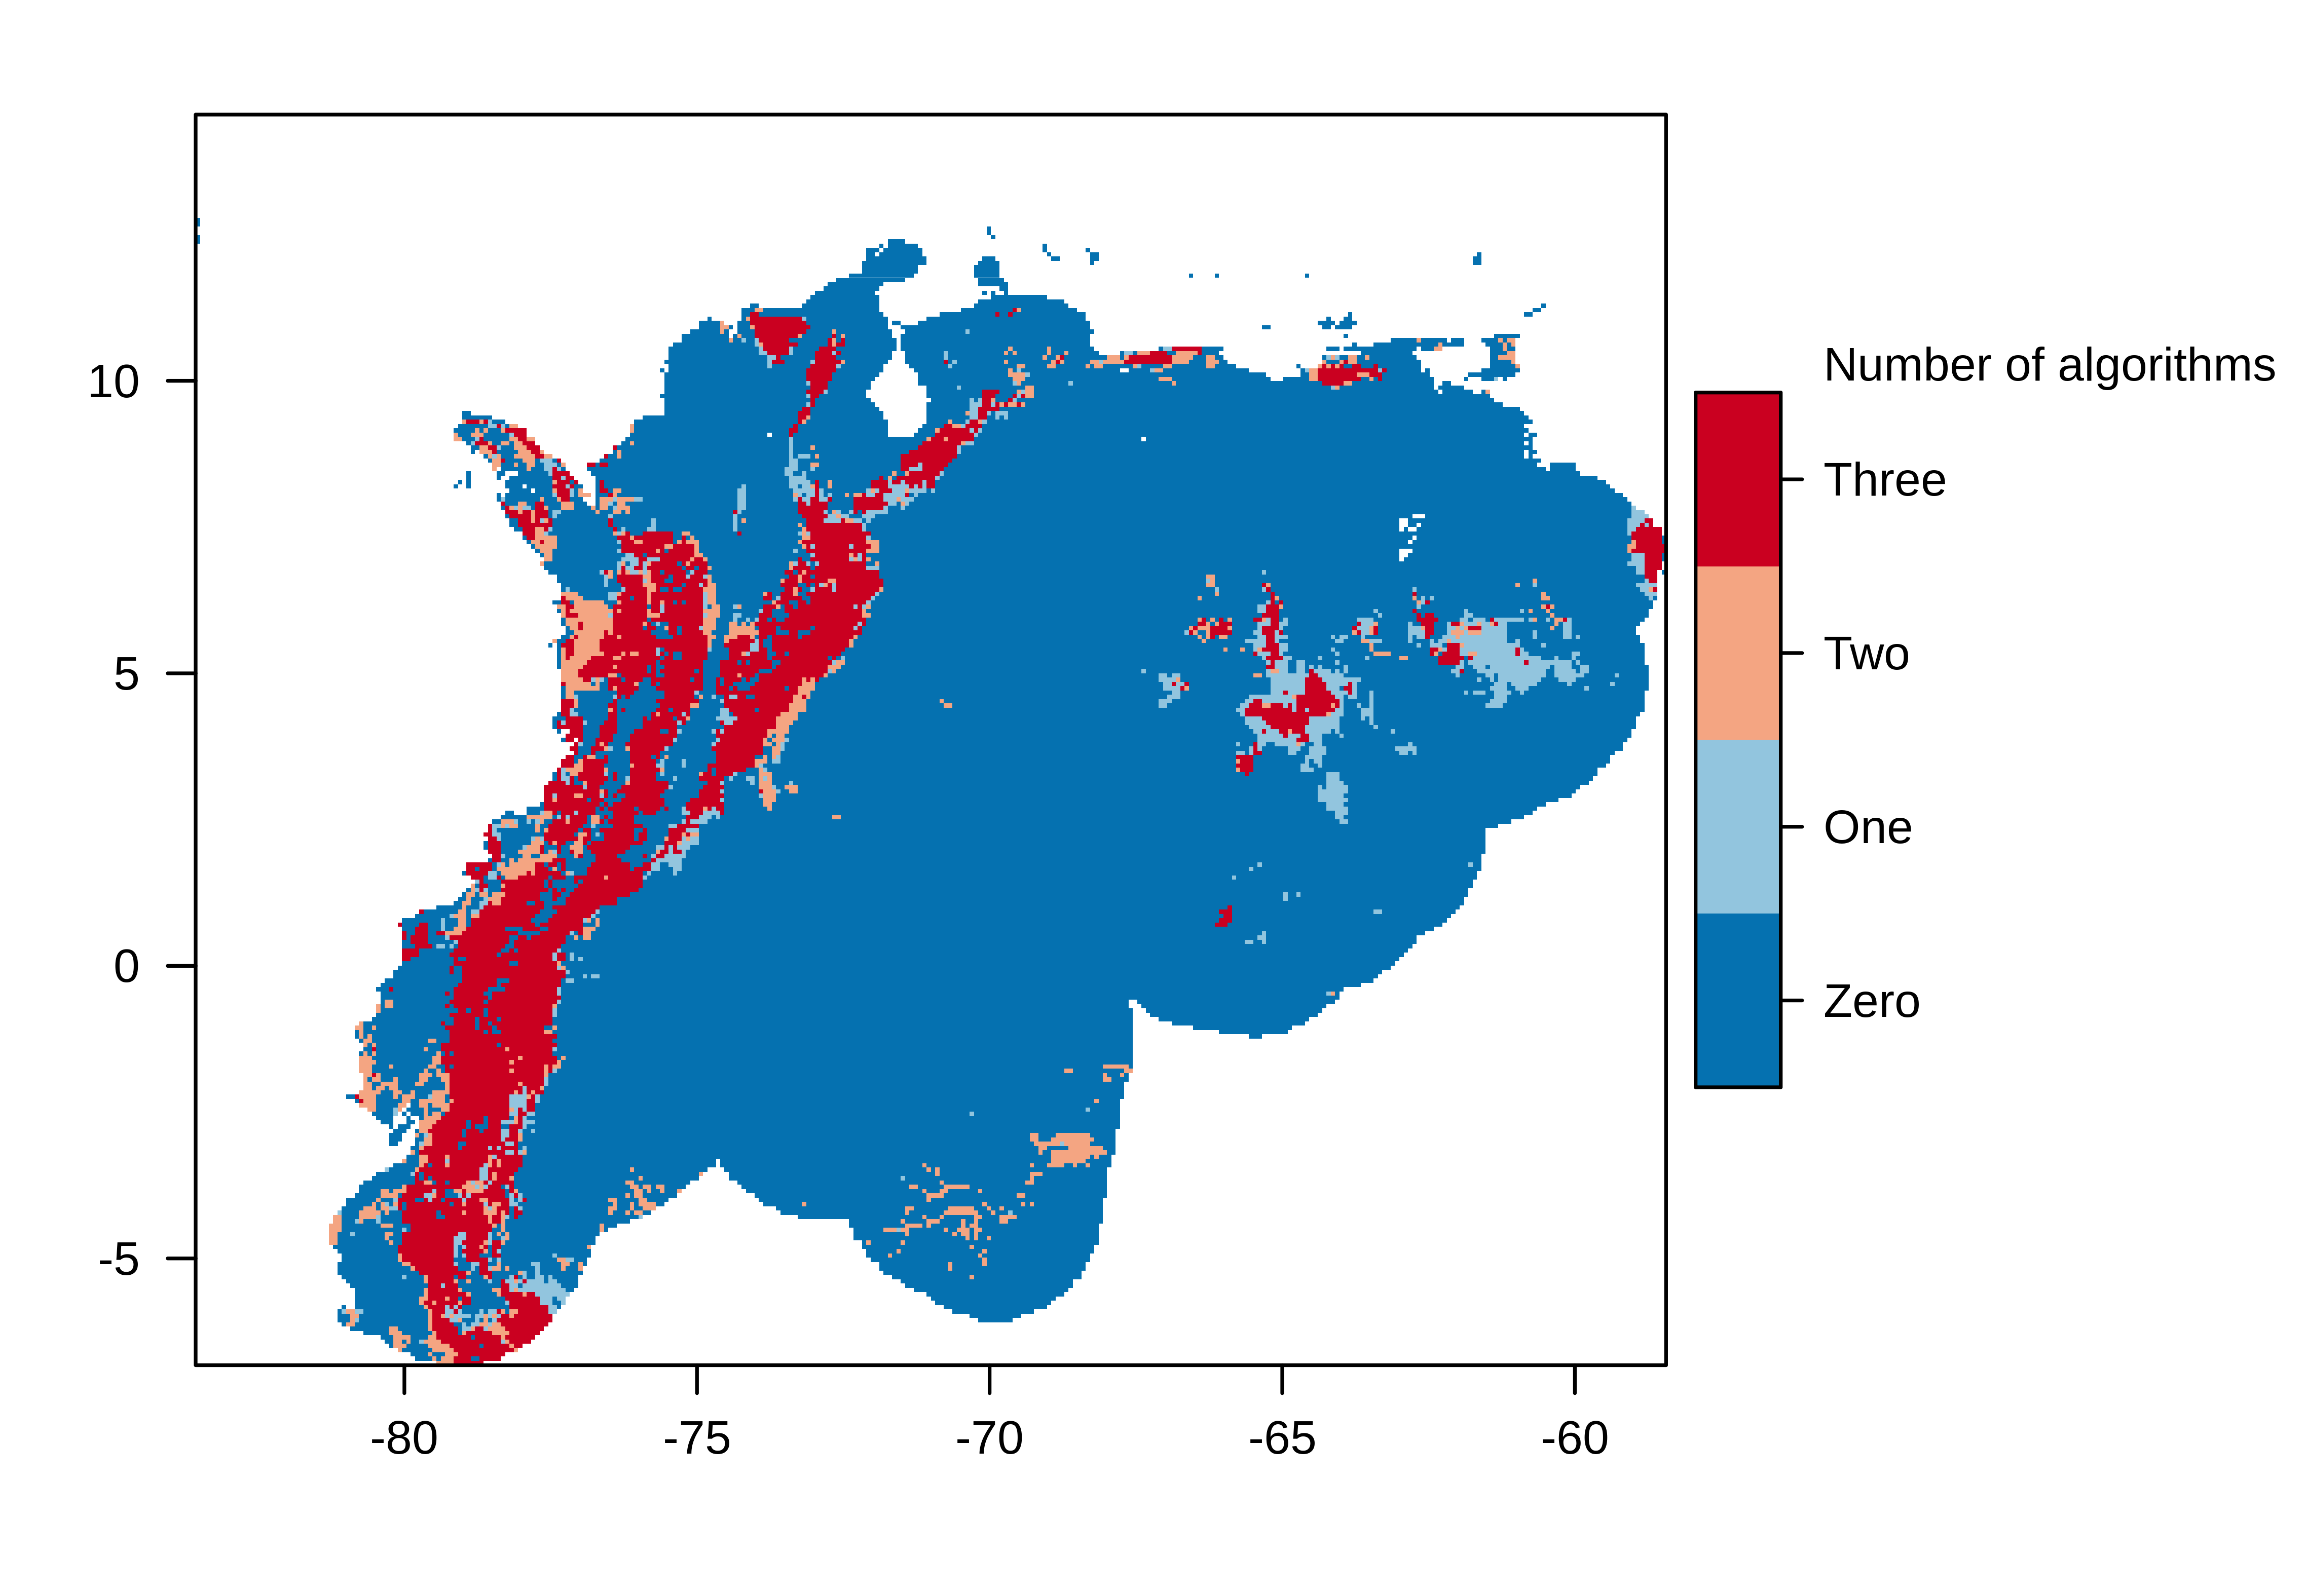
\includegraphics{NFPaper_files/figure-latex/NumberOfTimes-1.png}
\caption{\label{fig:NumberOfTimes}This map shows how many algorithms selected each cell}
\end{figure}

\hypertarget{correlation-comparison-spearman}{%
\subsubsection{Correlation comparison (Spearman)}\label{correlation-comparison-spearman}}

\begin{table}

\caption{\label{tab:Corr}Spearman correlation between the rank of the cells of all three methods}
\centering
\begin{tabular}[t]{lrrr}
\toprule
rowname & Linear.NF & Quadratic.NF & Zonation\\
\midrule
Linear.NF & NA & 0.9211996 & 0.6241322\\
Quadratic.NF & 0.9211996 & NA & 0.6690281\\
Zonation & 0.6241322 & 0.6690281 & NA\\
\bottomrule
\end{tabular}
\end{table}

\begin{figure}
\centering
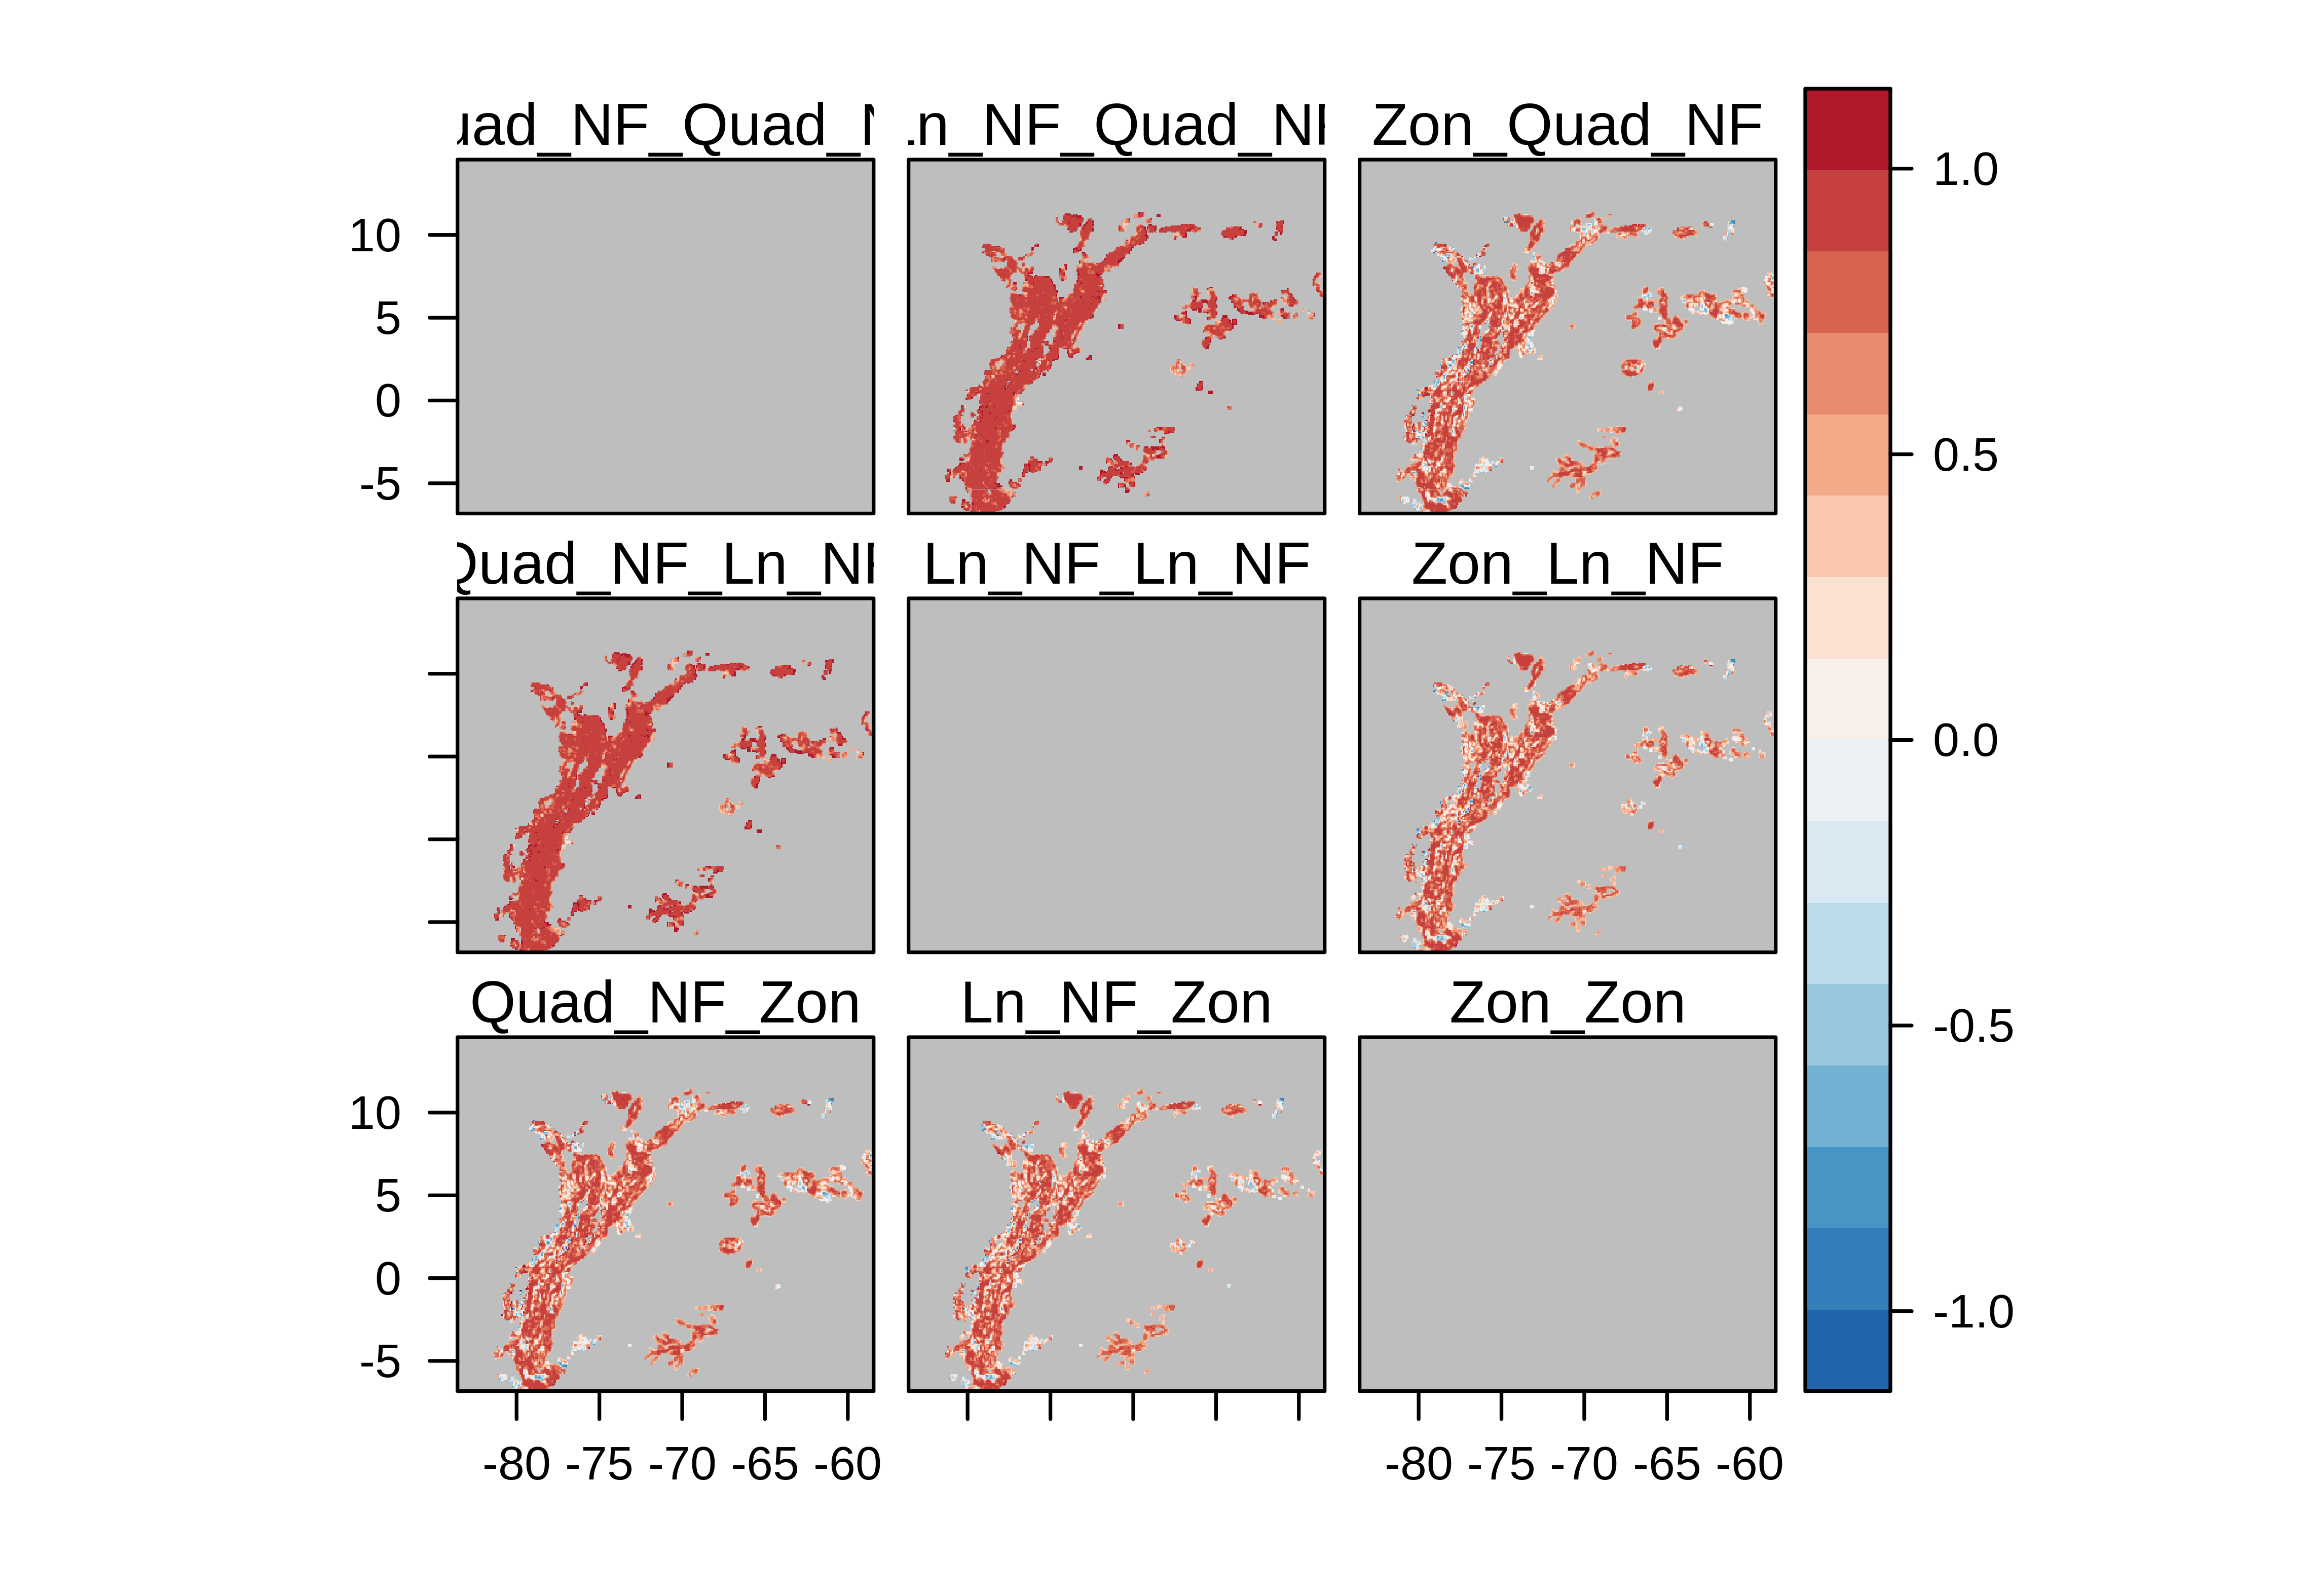
\includegraphics{NFPaper_files/figure-latex/LocalCorr-1.png}
\caption{\label{fig:LocalCorr}Box plot of local correlations between all three different methods of priorization}
\end{figure}

\begin{figure}
\centering
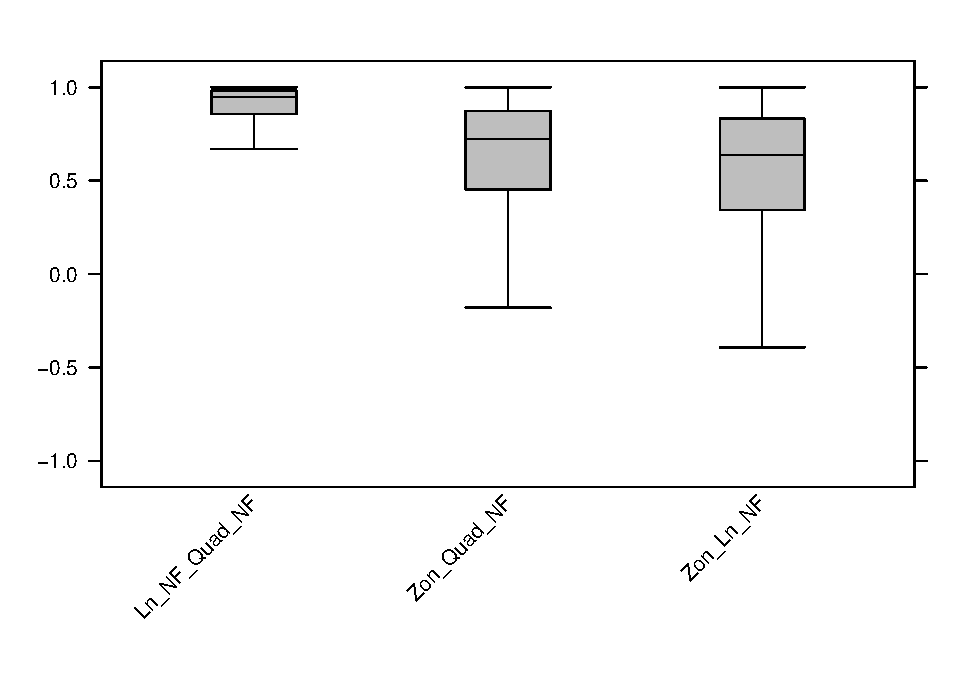
\includegraphics{NFPaper_files/figure-latex/Boxplot-1.pdf}
\caption{\label{fig:Boxplot}Box plot of local correlations between all three different methods of priorization}
\end{figure}

\hypertarget{discussion}{%
\section{Discussion}\label{discussion}}

\hypertarget{disclosureconflict-of-interest-statement}{%
\section*{Disclosure/Conflict-of-Interest Statement}\label{disclosureconflict-of-interest-statement}}
\addcontentsline{toc}{section}{Disclosure/Conflict-of-Interest Statement}

The authors declare that the research was conducted in the absence of any
commercial or financial relationships that could be construed as a potential
conflict of interest.

\hypertarget{author-contributions}{%
\section*{Author Contributions}\label{author-contributions}}
\addcontentsline{toc}{section}{Author Contributions}

When determining authorship the following criteria should be observed:

\begin{itemize}
\tightlist
\item
  Substantial contributions to the conception or design of the work; or the
  acquisition, analysis, or interpretation of data for the work; AND
\item
  Drafting the work or revising it critically for important intellectual
  content; AND
\item
  Final approval of the version to be published ; AND
\item
  Agreement to be accountable for all aspects of the work in ensuring that
  questions related to the accuracy or integrity of any part of the work are
  appropriately investigated and resolved.
\end{itemize}

Contributors who meet fewer than all 4 of the above criteria for authorship
should not be listed as authors, but they should be acknowledged.
(\url{http://www.icmje.org/roles_a.html})

The statement about the authors and contributors can be up to several sentences
long, describing the tasks of individual authors referred to by their initials
and should be included at the end of the manuscript before the References
section.

\hypertarget{acknowledgments}{%
\section*{Acknowledgments}\label{acknowledgments}}
\addcontentsline{toc}{section}{Acknowledgments}

Funding:

\hypertarget{supplemental-data}{%
\section{Supplemental Data}\label{supplemental-data}}

Supplementary Material should be uploaded separately on submission, if there are
Supplementary Figures, please include the caption in the same file as the
figure. LaTeX Supplementary Material templates can be found in the Frontiers
LaTeX folder

\hypertarget{references}{%
\section{References}\label{references}}

\hypertarget{figures}{%
\section*{Figures}\label{figures}}
\addcontentsline{toc}{section}{Figures}

\hypertarget{suplmentary-materials}{%
\section{Suplmentary materials}\label{suplmentary-materials}}

\hypertarget{list-of-species}{%
\subsection{List of species}\label{list-of-species}}

The species used for the solution were the folowing:

Aa maderoi, Abutilon ibarrense, Achyrocline crassiceps, Aciachne flagellifera, Aechmea drakeana, Aegiphila pennellii, Aequatorium sinuatifolium, Aequatorium verrucosum, Aetheolaena involucrata, Aetheolaena lingulata, Ageratina asclepiadea, Ageratina dendroides, Ageratina gynoxoides, Ageratina pseudochilca, Ageratina theaefolia, Ageratina vacciniaefolia, Agouticarpa grandistipula, Agrostis boyacensis, Agrostis foliata, Agrostis trichodes, Aiphanes grandis, Altensteinia virescens, Amazilia castaneiventris, Anagallis foemina, Anastrophyllum nigrescens, Andigena laminirostris, Anomobryum prostratum, Anotomys leander, Anredera brachystachys, Anthopterus schultzeae, Anthurium aristatum, Anthurium carchiense, Anthurium cordiforme, Anthurium flavolineatum, Anthurium giganteum, Anthurium gualeanum, Anthurium herthae, Anthurium lancea, Anthurium membranaceum, Anthurium morae, Anthurium palenquense, Anthurium pallatangense, Anthurium pedunculare, Anthurium pendulispadix, Anthurium phyllobaris, Anthurium rimbachii, Anthurium rugulosum, Anthurium wattii, Aphanactis jamesoniana, Aphanactis ollgaardii, Aphanactis piloselloides, Aragoa abietina, Aragoa cundinamarcensis, Aragoa occidentalis, Arcytophyllum aristatum, Arenaria venezuelana, Aristeguietia glutinosa, Arracacia moschata, Arremon phaeopleurus, Astragalus geminiflorus, Astragalus sprucei, Atlapetes flaviceps, Atlapetes leucopis, Atractus crassicaudatus, Atractus lasallei, Axinaea merianiae, Axinaea sodiroi, Azorella aretioides, Azorella cuatrecasasii, Azorella pedunculata, Baccharis revoluta, Baccharis rupicola, Baccharis teindalensis, Badilloa salicina, Bangsia aureocincta, Bangsia edwardsi, Bangsia rothschildi, Bartsia laticrenata, Bartsia orthocarpiflora, Bartsia santolinifolia, Bartsia stricta, Bauhinia stenantha, Begonia tiliifolia, Belloa radians, Berberis goudotii, Berberis hallii, Berberis rigidifolia, Berberis verticillata, Besleria angustiflora, Blakea glandulosa, Blakea hispida, Blakea oldemanii, Blakea rotundifolia, Bolborhynchus ferrugineifrons, Bomarea glaucescens, Bomarea linifolia, Bomarea patacocensis, Bomarea uncifolia, Brachtia andina, Brachyotum alpinum, Brachyotum confertum, Brachyotum fictum, Brachyotum gleasonii, Brachyotum harlingii, Brachyotum jamesonii, Brachyotum strigosum, Brayopsis colombiana, Breutelia squarrosa, Breutelia trianae, Browneopsis disepala, Brugmansia aurea, Brunellia boqueronensis, Brunellia colombiana, Bucquetia glutinosa, Buddleja pichinchensis, Burmeistera montipomum, Calamagrostis aurea, Calamagrostis effusa, Calamagrostis fibrovaginata, Calamagrostis guamanensis, Calamagrostis mollis, Calamagrostis podophora, Calceolaria dilatata, Calceolaria ferruginea, Calceolaria hyssopifolia, Calceolaria lamiifolia, Calceolaria pedunculata, Calceolaria purpurascens, Calceolaria rosmarinifolia, Calliergonella cuspidata, Campylopus argyrocaulon, Campylopus cleefii, Campylopus cucullatifolius, Campylopus edithae, Campylopus incertus, Campylopus pittieri, Campylopus subconcolor, Carex amicta, Casearia mexiae, Castilleja nubigena, Castratella piloselloides, Centradeniastrum album, Centropogon aequatorialis, Centropogon baezanus, Centropogon glabrifilis, Centropogon medusa, Centropogon nigricans, Centropogon subandinus, Cerastium floccosum, Ceratostema alatum, Cestrum peruvianum, Chalcostigma heteropogon, Chorisodontium speciosum, Chromolaena bullata, Chusquea subulata, Cinclodes excelsior, Cistothorus apolinari, Cistothorus meridae, Citharexylum sulcatum, Clavija eggersiana, Clethra crispa, Clinopodium nubigenum, Clinopodium taxifolium, Clinopodium tomentosum, Clusia callejasii, Coespeletia moritziana, Coespeletia spicata, Coespeletia thyrsiformis, Coespeletia timotensis, Colignonia pentoptera, Columnea albiflora, Columnea capillosa, Columnea ciliata, Columnea eubracteata, Conirostrum rufum, Conyza cardaminifolia, Conyza trihecatactis, Coursetia gracilis, Coussarea pilosiflora, Cranichis antioquiensis, Cranioleuca hellmayri, Critoniopsis occidentalis, Critoniopsis palaciosii, Critoniopsis sodiroi, Cronquistianthus niveus, Croton elegans, Croton rimbachii, Cryptotis equatoris, Culcitium nivale, Cyanolyca pulchra, Cynanchum microphyllum, Dalea humifusa, Dasyphyllum popayanense, Dendrophorbium lloense, Diglossa gloriosa, Diglossa gloriosissima, Diglossa indigotica, Diplostephium alveolatum, Diplostephium bicolor, Diplostephium cayambense, Diplostephium cinerascens, Diplostephium ericoides, Diplostephium frontinense, Diplostephium glandulosum, Diplostephium hartwegii, Diplostephium ochraceum, Diplostephium phylicoides, Diplostephium revolutum, Diplostephium rhododendroides, Diplostephium rhomboidale, Diplostephium rupestre, Diplostephium schultzii, Diplostephium spinulosum, Diplostephium tenuifolium, Diplostephium tolimense, Diplostephium violaceum, Diplostichum longirostre, Distichia acicularis, Ditrichum submersum, Draba aretioides, Draba hallii, Draba obovata, Draba splendens, Draba spruceana, Dracula sodiroi, Drepanocladus exannulatus, Drymonia crenatiloba, Drymonia laciniosa, Dysithamnus occidentalis, Elaphoglossum antisanae, Elaphoglossum heliconiifolium, Elaphoglossum yatesii, Elasis hirsuta, Elatine ecuadoriensis, Elleanthus gastroglottis, Elleanthus petrogeiton, Epidendrum englerianum, Epidendrum marsupiale, Epidendrum pallatangae, Epidendrum pichinchae, Epidendrum porphyreum, Eragrostis condensata, Erigeron ecuadoriensis, Eriocnemis cupreoventris, Eriocnemis derbyi, Eriocnemis mosquera, Eryngium humboldtii, Espeletia argentea, Espeletia barclayana, Espeletia batata, Espeletia boyacensis, Espeletia brassicoidea, Espeletia cleefii, Espeletia congestiflora, Espeletia conglomerata, Espeletia frontinoensis, Espeletia grandiflora, Espeletia hartwegiana, Espeletia killipii, Espeletia lopezii, Espeletia murilloi, Espeletia pycnophylla, Espeletia schultesiana, Espeletia schultzii, Espeletia semiglobulata, Espeletia summapacis, Espeletia tunjana, Espeletia uribei, Espeletiopsis colombiana, Espeletiopsis corymbosa, Espeletiopsis pannosa, Espeletiopsis petiolata, Eudema nubigena, Euphonia concinna, Festuca andicola, Festuca chimborazensis, Festuca glumosa, Festuca subulifolia, Festuca vaginalis, Fuchsia ampliata, Fuchsia caucana, Fuchsia dependens, Fuchsia hartwegii, Fuchsia macrostigma, Fuchsia orientalis, Fuchsia sessilifolia, Fuchsia sylvatica, Fuchsia vulcanica, Gasteranthus columbianus, Gasteranthus lateralis, Gasteranthus leopardus, Gasteranthus quitensis, Gaultheria cordifolia, Geissanthus argutus, Genista monspessulana, Gentianella cerastioides, Gentianella cernua, Gentianella corymbosa, Gentianella foliosa, Gentianella hirculus, Gentianella hyssopifolia, Gentianella nummulariifolia, Gentianella rapunculoides, Gentianella rupicola, Geonoma divisa, Geranium maniculatum, Geranium multiceps, Geranium multipartitum, Glaucidium nubicola, Gongylolepis jauaensis, Grallaria alleni, Grallaria flavotincta, Grallaria milleri, Grallaria rufocinerea, Grallaricula lineifrons, Grallaricula loricata, Grosvenoria hypargyra, Grosvenoria rimbachii, Gustavia longifuniculata, Gustavia serrata, Guzmania jaramilloi, Guzmania lehmanniana, Guzmania vanvolxemii, Guzmania wittmackii, Gynoxys acostae, Gynoxys hirsuta, Gynoxys laurata, Gynoxys miniphylla, Gynoxys parvifolia, Gynoxys pendula, Gynoxys sodiroi, Gynoxys stuebelii, Gynoxys tolimensis, Halenia adpressa, Halenia gentianoides, Halenia pulchella, Haplophaedia lugens, Hebeclinium tetragonum, Hedyosmum parvifolium, Heliangelus strophianus, Heliconia dielsiana, Heppiella verticillata, Hesperomeles goudotiana, Hieracium avilae, Huperzia capellae, Huperzia cruenta, Huperzia cumingii, Huperzia hystrix, Huperzia lindenii, Huperzia llanganatensis, Huperzia polydactyla, Huperzia rufescens, Huperzia transilla, Huperzia unguiculata, Hypericum decandrum, Hypericum goyanesii, Hypericum myricariifolium, Hypericum prostratum, Hypericum quitense, Hypochaeris setosa, Inga extra-nodis, Isoetes andina, Isoetes bischlerae, Isoetes boyacensis, Isoetes novo-granadensis, Isoetes palmeri, Jamesonia bogotensis, Jamesonia cinnamomea, Jamesonia pulchra, Juncus breviculmis, Juncus echinocephalus, Juncus ecuadoriensis, Lachemilla angustata, Lachemilla hirta, Lachemilla hispidula, Lachemilla holosericea, Lachemilla jamesonii, Lachemilla nivalis, Lachemilla rupestris, Lachemilla tanacetifolia, Lasiocephalus ovatus, Ledothamnus luteus, Lepanthes effusa, Lepanthes pilosella, Lepechinia vulcanicola, Lepidozia macrocolea, Leptodontium erythroneuron, Leptoscyphus cleefii, Leptotila conoveri, Liabum saloyense, Llerasia hypoleuca, Loricaria antisanensis, Loricaria complanata, Loricaria ilinissae, Lourteigia humilis, Lourteigia microphylla, Lupinus alopecuroides, Lupinus colombiensis, Lupinus smithianus, Lysipomia montioides, Lysipomia muscoides, Macleania bullata, Macleania coccoloboides, Macleania cordifolia, Macleania ericae, Macleania loeseneriana, Macrocarpaea glabra, Margarornis stellatus, Masdevallia ophioglossa, Matisia palenquiana, Mauritiella macroclada, Melothria longituba, Melpomene assurgens, Melpomene sodiroi, Meriania heptamera, Meriania hernandoi, Metallura baroni, Metallura williami, Mezobromelia lyman-smithii, Miconia aguirrei, Miconia biappendiculata, Miconia chlorocarpa, Miconia dielsii, Miconia glandulistyla, Miconia hymenanthera, Miconia nodosa, Miconia pernettifolia, Miconia pichinchensis, Miconia psychrophila, Miconia scutata, Miconia summa, Miconia turgida, Mimosa quitensis, Mimosa townsendii, Mona meridensis, Monnina crassifolia, Monnina equatoriensis, Monnina obtusifolia, Monnina pseudopilosa, Monnina revoluta, Monnina sodiroana, Monnina tenuifolia, Monticalia arbutifolia, Monticalia peruviana, Monticalia vaccinioides, Morella singularis, Muscisaxicola alpinus, Mutisia grandiflora, Mutisia microphylla, Mutisia sodiroi, Myioborus albifrons, Myrrhidendron glaucescens, Myrsine panamensis, Niphogeton azorelloides, Niphogeton glaucescens, Niphogeton josei, Notopleura marginata, Nototriche jamesonii, Nototriche phyllanthos, Odontoglossum hallii, Odontophorus atrifrons, Odontophorus melanonotus, Oncidium serratum, Opuntia soederstromiana, Oreobolus cleefii, Oreopanax corazonensis, Oreopanax ecuadorensis, Oreopanax ellsworthii, Oreopanax grandifolius, Oreopanax mutisianus, Oreopanax nigrum, Oreopanax palamophyllus, Oreopanax ruizanus, Oreothraupis arremonops, Oreotrochilus chimborazo, Ossaea sessilifolia, Oxypogon guerinii, Paepalanthus alpinus, Paepalanthus karstenii, Paepalanthus lodiculoides, Palicourea prodiga, Palicourea sodiroi, Palicourea subalatoides, Pappobolus imbaburensis, Paspalum hirtum, Passiflora adulterina, Passiflora crispolanata, Passiflora cuatrecasasii, Passiflora jamesonii, Passiflora roseorum, Passiflora trinervia, Pedicularis incurva, Pentacalia abietina, Pentacalia americana, Pentacalia arbutifolia, Pentacalia flosfragrans, Pentacalia guadalupe, Pentacalia ledifolia, Pentacalia nitida, Pentacalia pulchella, Pentacalia reissiana, Pentacalia vaccinioides, Pentacalia vernicosa, Pentagonia grandiflora, Peperomia fuscipunctata, Peperomia miqueliana, Pernettya hirta, Phalcoboenus carunculatus, Philodendron oligospermum, Philodendron rugosum, Philonotis andina, Pilea gallowayana, Pinguicula elongata, Piper laguna-cochanum, Piper sodiroi, Piper subflavum, Pipreola jucunda, Pitcairnia commixta, Pitcairnia cosangaensis, Pitcairnia fusca, Pittosporum undulatum, Plagiocheilus frigidus, Plagiocheilus solivaeformis, Pleurothallis ensata, Pleurothallis macra, Pleurothallis truncata, Plutarchia guascensis, Poa cucullata, Poa paramoensis, Poa pauciflora, Polylepis lanuginosa, Polylepis quadrijuga, Polylepis reticulata, Polypodium mindense, Polypodium monosorum, Polypodium segregatum, Polytrichadelphus ciliatus, Pouteria capacifolia, Prunus antioquensis, Prunus herthae, Psammisia debilis, Psammisia occidentalis, Psammisia sclerantha, Psychotria boqueronensis, Psychotria cuatrecasasii, Puya glomerifera, Puya goudotiana, Puya nitida, Puya santosii, Puya trianae, Pyrrhura hoematotis, Racinaea subalata, Rallus semiplumbeus, Ranunculus nubigenus, Renealmia fragilis, Renealmia sessilifolia, Rhodospatha densinervia, Rhodostemonodaphne laxa, Rhynchospora paramora, Ribes hirtum, Ribes lehmannii, Rubus choachiensis, Rubus gachetensis, Ruilopezia atropurpurea, Ruilopezia marcescens, Rumex tolimensis, Saguinus leucopus, Salvia pichinchensis, Saurauia chiliantha, Saurauia crassisepala, Saurauia omichlophila, Saurauia peduncularis, Saurauia pseudostrigillosa, Schefflera acaropunctata, Schefflera lasiogyne, Schefflera marginata, Schefflera ramosissima, Scorpidium scorpioides, Scytalopus griseicollis, Scytalopus rodriguezi, Scytalopus vicinior, Senecio culcitioides, Senecio formosoides, Senecio hypsobates, Senecio leucanthemoides, Senecio madagascariensis, Senecio niveoaureus, Senecio subruncinatus, Setaria cernua, Siparuna croatii, Siparuna palenquensis, Siphocampylus affinis, Siphocampylus brevicalyx, Siphocampylus columnae, Solanum crinitipes, Solanum paucijugum, Sorocea sarcocarpa, Sparrmannia africana, Sphaeradenia hamata, Sphaeradenia horrida, Sphagnum compactum, Sphagnum oxyphyllum, Sphyrospermum boekei, Sphyrospermum grandifolium, Sporobolus bogotensis, Stachys bogotensis, Stachys elliptica, Stelis columnaris, Stelis piperina, Stellaria recurvata, Stenospermation longifolium, Stilpnophyllum grandifolium, Stilpnophyllum oellgaardii, Stipa milleana, Stipa rosea, Symphyogyna bogotensis, Symplocos cundinamarcensis, Symplocos rhomboidea, Symplocos theiformis, Synallaxis castanea, Synallaxis subpudica, Syntrichia andicola, Tagetes zypaquirensis, Tangara rufigenis, Telipogon nervosus, Ternstroemia cleistogama, Terpsichore heteromorpha, Terpsichore pichinchae, Tetragastris varians, Thelypteris rigescens, Themistoclesia epiphytica, Theobroma gileri, Thibaudia andrei, Thibaudia grantii, Thibaudia parvifolia, Thomasomys hylophilus, Thomasomys niveipes, Thryophilus nicefori, Tibouchina gleasoniana, Tibouchina paleacea, Tibouchina pendula, Tillandsia emergens, Tillandsia incarnata, Tillandsia lajensis, Tillandsia secunda, Tillandsia superba, Tillandsia truncata, Tournefortia ramosissima, Uncinia paludosa, Uniola condensata, Urothraupis stolzmanni, Urtica longispica, Valeriana adscendens, Valeriana arborea, Valeriana bracteata, Valeriana tatamana, Valeriana tomentosa, Verbesina brachypoda, Verbesina latisquama, Verbesina lloensis, Verbesina sodiroi, Viburnum anabaptista, Viburnum antioquiense, Vigna venusta, Viola glandularis, Vireo masteri, Weinmannia polyphylla, Wettinia anomala, Xenophyllum crassum, Zanthoxylum lepidopteriphilum, Zygodon pichinchensis

\hypertarget{refs}{}
\leavevmode\hypertarget{ref-Ahuja93}{}%
Ahuja, R. K., Magnanti, T. L., \& Orlin, J. B. (1993). \emph{Network flows: Theory, algorithms, and applications}. Englewood Cliffs, NJ: Prentice Hall.

\leavevmode\hypertarget{ref-alagador2014shifting}{}%
Alagador, D., Cerdeira, J. O., \& Araújo, M. B. (2014). Shifting protected areas: Scheduling spatial priorities under climate change. \emph{Journal of Applied Ecology}, \emph{51}(3), 703--713.

\leavevmode\hypertarget{ref-araujo2004would}{}%
Araújo, M. B., Cabeza, M., Thuiller, W., Hannah, L., \& Williams, P. H. (2004). Would climate change drive species out of reserves? An assessment of existing reserve-selection methods. \emph{Global Change Biology}, \emph{10}(9), 1618--1626.

\leavevmode\hypertarget{ref-baker2014linking}{}%
Baker, M. E., Rycroft, S., \& Smith, V. S. (2014). Linking multiple biodiversity informatics platforms with darwin core archives. \emph{Biodiversity Data Journal}, (2).

\leavevmode\hypertarget{ref-beier2007linkage}{}%
Beier, P., Majka, D., \& Bayless, T. (2007). Linkage designs for arizona's missing linkages. \emph{Arizona Game and Fish Department, Phoenix}.

\leavevmode\hypertarget{ref-Boyle2019GNRS}{}%
Boyle, B. (2019a). Geographic name resolution service (gnrs). \emph{GitHub repository}. \url{https://github.com/ojalaquellueva/gnrs}; GitHub.

\leavevmode\hypertarget{ref-Boyle2019NSR}{}%
Boyle, B. (2019b). Native status resolver (nsr). \emph{GitHub repository}. \url{https://github.com/ojalaquellueva/nsr}; GitHub.

\leavevmode\hypertarget{ref-boyle2013taxonomic}{}%
Boyle, B., Hopkins, N., Lu, Z., Garay, J. A. R., Mozzherin, D., Rees, T., \ldots{} others. (2013). The taxonomic name resolution service: An online tool for automated standardization of plant names. \emph{BMC Bioinformatics}, \emph{14}(1), 16.

\leavevmode\hypertarget{ref-chen2011rapid}{}%
Chen, I.-C., Hill, J. K., Ohlemüller, R., Roy, D. B., \& Thomas, C. D. (2011). Rapid range shifts of species associated with high levels of climate warming. \emph{Science}, \emph{333}(6045), 1024--1026.

\leavevmode\hypertarget{ref-Corcoran_Quadcost}{}%
Corcoran, D., \& Fajardo, J. (2019). \emph{QuadCostAmpl: Transforms a stack of timeslices of species distribution models into data for ampl modeling}. Retrieved from \url{https://github.com/derek-corcoran-barrios/QuadCostAmpl}

\leavevmode\hypertarget{ref-cushman2013biological}{}%
Cushman, S. A., McRae, B., Adriaensen, F., Beier, P., Shirley, M., \& Zeller, K. (2013). Biological corridors and connectivity {[}chapter 21{]}. \emph{In: Macdonald, DW; Willis, KJ, Eds. Key Topics in Conservation Biology 2. Hoboken, NJ: Wiley-Blackwell. P. 384-404.}, 384--404.

\leavevmode\hypertarget{ref-de2018soilgrids}{}%
De Sousa, L., Heuvelink, G., Batjes, N., \& Kempen, B. (2018). SoilGrids: Using big data solutions and machine learning algorithms for global soil mapping. In \emph{Scientific symposium fair data sciences for green life sciences} (pp. 1--1).

\leavevmode\hypertarget{ref-di2014quick}{}%
Di Minin, E., Veach, V., Lehtomäki, J., Montesino Pouzols, F., Moilanen, A., \& others. (2014). A quick introduction to zonation.

\leavevmode\hypertarget{ref-fajardo_javier_2018_2669407}{}%
Fajardo, J., Corcoran, D., Roehrdanz, P., Hannah, L., \& Marquet, P. (2018, October). doi:\href{https://doi.org/10.5281/zenodo.2669407}{10.5281/zenodo.2669407}

\leavevmode\hypertarget{ref-gregory2014forecasts}{}%
Gregory, S. D., Ancrenaz, M., Brook, B. W., Goossens, B., Alfred, R., Ambu, L. N., \& Fordham, D. A. (2014). Forecasts of habitat suitability improve habitat corridor efficacy in rapidly changing environments. \emph{Diversity and Distributions}, \emph{20}(9), 1044--1057.

\leavevmode\hypertarget{ref-hannah2007protected}{}%
Hannah, L., Midgley, G., Andelman, S., Araújo, M., Hughes, G., Martinez-Meyer, E., \ldots{} Williams, P. (2007). Protected area needs in a changing climate. \emph{Frontiers in Ecology and the Environment}, \emph{5}(3), 131--138.

\leavevmode\hypertarget{ref-Hanson2019}{}%
Hanson, J. O., Schuster, R., Morrell, N., Strimas-Mackey, M., Watts, M. E., Arcese, P., \ldots{} Possingham, H. P. (2019). \emph{Prioritizr: Systematic conservation prioritization in r}. Retrieved from \url{https://CRAN.R-project.org/package=prioritizr}

\leavevmode\hypertarget{ref-Hijmans_Dismo}{}%
Hijmans, R. J., Phillips, S., Leathwick, J., \& Elith, J. (2017). \emph{Dismo: Species distribution modeling}. Retrieved from \url{https://CRAN.R-project.org/package=dismo}

\leavevmode\hypertarget{ref-jenkins2015us}{}%
Jenkins, C. N., Van Houtan, K. S., Pimm, S. L., \& Sexton, J. O. (2015). US protected lands mismatch biodiversity priorities. \emph{Proceedings of the National Academy of Sciences}, \emph{112}(16), 5081--5086.

\leavevmode\hypertarget{ref-jones2016incorporating}{}%
Jones, K. R., Watson, J. E., Possingham, H. P., \& Klein, C. J. (2016). Incorporating climate change into spatial conservation prioritisation: A review. \emph{Biological Conservation}, \emph{194}, 121--130.

\leavevmode\hypertarget{ref-lawler2013projected}{}%
Lawler, J., Ruesch, A., Olden, J., \& McRae, B. (2013). Projected climate-driven faunal movement routes. \emph{Ecology Letters}, \emph{16}(8), 1014--1022.

\leavevmode\hypertarget{ref-lenoir2008significant}{}%
Lenoir, J., Gégout, J.-C., Marquet, P., De Ruffray, P., \& Brisse, H. (2008). A significant upward shift in plant species optimum elevation during the 20th century. \emph{Science}, \emph{320}(5884), 1768--1771.

\leavevmode\hypertarget{ref-merow2014we}{}%
Merow, C., Smith, M. J., Edwards Jr, T. C., Guisan, A., McMahon, S. M., Normand, S., \ldots{} Elith, J. (2014). What do we gain from simplicity versus complexity in species distribution models? \emph{Ecography}, \emph{37}(12), 1267--1281.

\leavevmode\hypertarget{ref-merow2013practical}{}%
Merow, C., Smith, M. J., \& Silander Jr, J. A. (2013). A practical guide to maxent for modeling species' distributions: What it does, and why inputs and settings matter. \emph{Ecography}, \emph{36}(10), 1058--1069.

\leavevmode\hypertarget{ref-naidoo2007global}{}%
Naidoo, R., \& Iwamura, T. (2007). Global-scale mapping of economic benefits from agricultural lands: Implications for conservation priorities. \emph{Biological Conservation}, \emph{140}(1-2), 40--49.

\leavevmode\hypertarget{ref-nunez2013connectivity}{}%
Nuñez, T. A., Lawler, J. J., McRae, B. H., Pierce, D. J., Krosby, M. B., Kavanagh, D. M., \ldots{} Tewksbury, J. J. (2013). Connectivity planning to address climate change. \emph{Conservation Biology}, \emph{27}(2), 407--416.

\leavevmode\hypertarget{ref-phillips2006maximum}{}%
Phillips, S. J., Anderson, R. P., \& Schapire, R. E. (2006). Maximum entropy modeling of species geographic distributions. \emph{Ecological Modelling}, \emph{190}(3-4), 231--259.

\leavevmode\hypertarget{ref-phillips2008optimizing}{}%
Phillips, S. J., Williams, P., Midgley, G., \& Archer, A. (2008). Optimizing dispersal corridors for the cape proteaceae using network flow. \emph{Ecological Applications}, \emph{18}(5), 1200--1211.

\leavevmode\hypertarget{ref-regos2016predicting}{}%
Regos, A., D'Amen, M., Titeux, N., Herrando, S., Guisan, A., \& Brotons, L. (2016). Predicting the future effectiveness of protected areas for bird conservation in mediterranean ecosystems under climate change and novel fire regime scenarios. \emph{Diversity and Distributions}, \emph{22}(1), 83--96.

\leavevmode\hypertarget{ref-rodrigues2004effectiveness}{}%
Rodrigues, A. S., Andelman, S. J., Bakarr, M. I., Boitani, L., Brooks, T. M., Cowling, R. M., \ldots{} others. (2004). Effectiveness of the global protected area network in representing species diversity. \emph{Nature}, \emph{428}(6983), 640.

\leavevmode\hypertarget{ref-rosenberg1997biological}{}%
Rosenberg, D. K., Noon, B. R., \& Meslow, E. C. (1997). Biological corridors: Form, function, and efficacy. \emph{BioScience}, \emph{47}(10), 677--687.

\leavevmode\hypertarget{ref-tuanmu2014global}{}%
Tuanmu, M.-N., \& Jetz, W. (2014). A global 1-km consensus land-cover product for biodiversity and ecosystem modelling. \emph{Global Ecology and Biogeography}, \emph{23}(9), 1031--1045.

\leavevmode\hypertarget{ref-unep2018ngs}{}%
UNEP-WCMC, I. (2018). NGS (2018). \emph{Protected Planet Report}.

\leavevmode\hypertarget{ref-williams2005planning}{}%
Williams, P., Hannah, L., Andelman, S., Midgley, G., Araújo, M., Hughes, G., \ldots{} Pearson, R. (2005). Planning for climate change: Identifying minimum-dispersal corridors for the cape proteaceae. \emph{Conservation Biology}, \emph{19}(4), 1063--1074.

\leavevmode\hypertarget{ref-zappa2017storylines}{}%
Zappa, G., \& Shepherd, T. G. (2017). Storylines of atmospheric circulation change for european regional climate impact assessment. \emph{Journal of Climate}, \emph{30}(16), 6561--6577.


\end{document}
